\documentclass[pdftex,12pt,a4paper]{report}

\usepackage[portuguese,english]{babel}
\usepackage[T1]{fontenc} 
\usepackage[utf8]{inputenc}
\usepackage[pdftex]{graphicx}
\usepackage{minitoc}
\usepackage{hyperref}
\usepackage{indentfirst}
\usepackage[compact]{titlesec}
\usepackage{fancyhdr}
\usepackage{caption}
\usepackage{pgfplots}
\usepackage{pgfplotstable}
\usepackage{fixltx2e}
\usepackage{mathtools}
\usepackage{fancyhdr}
\usepackage{listings}
\usepackage{color}
\usepackage{sverb}

\definecolor{Black}{rgb}{0.0, 0.0, 0.0}
\definecolor{Blue}{rgb}{0.0, 0.0, 1.0}
\definecolor{DarkGreen}{rgb}{0.0, 0.42, 0.24}
\definecolor{Red}{rgb}{0.89, 0.0, 0.13}

\lstset{
  breaklines=true,                                     % line wrapping on
  language=SQL,
  frame=ltrb,
  framesep=5pt,
  basicstyle=\normalsize,
  keywordstyle=\ttfamily\color{Blue},
  identifierstyle=\ttfamily\color{Black}\bfseries,
  commentstyle=\color{DarkGreen},
  stringstyle=\ttfamily\color{Red},
  showstringspaces=ture
}

\pagestyle{fancy}
\renewcommand*\thesection{\thechapter\arabic{section}}
\newcommand{\HRule}{\rule{\linewidth}{0.5mm}}
\begin{document}

\begin{titlepage}

\begin{center}


\includegraphics[width=0.15\textwidth]{./logo}\\[0.5cm]    

\textsc{\large Universidade de Aveiro \\[1cm]\large departamento de electrónica, telecomunicações e informática}\\[1cm]

\textsc{\large{42532}\large - Base de Dados \\[1cm]}

\HRule \\[0.5cm]
{ \huge \bfseries Football Club}\\[0.4cm]
{ \large \bfseries Trabalho Prático Final}\\[0.4cm]
\HRule \\[1cm]

\textsc{\small{8240 - MESTRADO INTEGRADO EM ENGENHARIA DE COMPUTADORES E TELEMÁTICA}}\\[1cm]

\begin{minipage}{0.4\textwidth}

\begin{flushleft} \large
\href{mailto:rafael.ferreira@ua.pt}{António Rafael da \\ Costa Ferreira }
 \small{\\NMec: 67405 | P4G5}
\end{flushleft}
\end{minipage}
\begin{minipage}{0.4\textwidth}

\begin{flushright} \large
\href{mailto:rodrigocunha@ua.pt}{Rodrigo Lopes \\ da Cunha}
\small{\\NMec: 67800 | P4G5}
\end{flushright}
\end{minipage}\\[1cm]

{\large Docente: Carlos Manuel Azevedo Costa   }\\[0.5cm]

\vfill

{\large Junho de 2015 \\ 2014-2015}

\end{center}

\end{titlepage} %Titulo do Relatorio
\renewcommand{\headrulewidth}{0pt}

%Cabeçalhos de rodapé
\fancyhead{}
\fancyfoot{}
\lhead{Football Club - Trabalho Prático Final}
\rhead{BD - 2014/2015}
\lfoot{\textit{P4G5} \\ Rafael Ferreira nmec: 67405 \\ Rodrigo Cunha nmec: 67800}
\rfoot{\thepage}

%Renomear Comandos
\renewcommand*\contentsname{Conteúdos}
\renewcommand*\figurename{Figura}
\renewcommand*\tablename{Tabela}

%Conteúdos, dar paragrafo
\tableofcontents
%Headers
\renewcommand{\headrulewidth}{0.15pt}
\renewcommand{\thechapter}{}

\clearpage

\section{Introdução}
% o que, porquê e o objetivo
O trabalho proposto para o projeto da unidade curricular de Base de Dados é uma plataforma de gestão de um clube de futebol. Usando os conhecimentos adquiridos, propôs-se o desenvolvimento deste projeto visto que o futebol é uma modalidade mundial, envolvendo vários tipos de interesse. 

O objetivo desta base de dados desenvolvida é permitir a gestão de todos os processos de um clube de futebol, como será visto mais à frente.

Além de se ter desenvolvido esta base de dados, desenvolveu-se uma aplicação WPF C\# para permitir a manipulação dos dados da base de dados de forma mais simplificada para um utilizador final.

Esta base de dados deve fornecer ferramentas que permitam a criação, remoção, alteração e consulta da base de dados de forma segura, eficiente e robusta.

O relatório reflete todos os passos e decisões tomadas na criação da base de dados que sustenta o projeto bem como uma descrição das capacidades da aplicação desenvolvida para o cliente.

Para a criação deste projeto foi seguido o processo leccionado nas aulas, sendo estas as seguintes fases do processo: análise de requisitos, desenho conceptual, desenho do esquema lógico, desenho do esquema físico e administração.

\newpage
\section{Análise de Requisitos}

A análise de requisitos foi uma das partes mais importantes do processo de concepção do projeto uma vez que ajudou a ter uma visão clara do que o sistema teria de suportar. Após realizado um "brainstorming", estas são as características que o sistema deve suportar:

Uma \textbf{pessoa} é identificada por um nome, B.I. (sendo que este B.I. é único), endereço, NIF, Sexo, Data de Nascimento e Nacionalidade. Esta pessoa pode ser uma Pessoa que pertença ao pessoal interno do clube (Staff) ou ser sócio do clube. 

Uma \textbf{pessoa interna} ao clube tem salário e um ID que é automaticamente atribuído e o identifica dentro do clube.

Um \textbf{sócio do clube} tem um nº de sócio, o ano até que as suas cotas estão pagas (são cotas anuais) e um valor de cotas que tem de pagar todos os anos. Um sócio pode ter ou não um \textbf{lugar anual}, tendo este, um valor, data de início, duração, Nº Lugar e Nº Fila e ID da secção.

Um \textbf{lugar} tem um nº de lugar e fila. Uma \textbf{secção} tem um ID de secção e tipo. 

Um \textbf{jogador} é uma pessoa interna ao clube e é identificado com um ID da federação, peso e altura. Este joga em equipas do clube.

Um \textbf{treinador} é uma pessoa interna do clube e é identificado com um ID da federação e cargo. Este tem equipas do clube.

Uma \textbf{equipa} tem uma idade máxima de jogadores que podem pertencer à mesma e um nome único.

Uma equipa pode ter \textbf{treinos} que são caracterizados por uma data e uma hora e são realizados num determinado campo.

Um \textbf{campo} tem um endereço e um ID.

Uma pessoa interna ao clube (\textbf{Staff}) tem um cargo e pode trabalhar um Departamento.

Um \textbf{departamento} tem um endereço, ID de departamento e um nome.

\newpage

Foram também registadas algumas especificações para o desenho conceptual:

- Uma pessoa pode ser um sócio e uma pessoa interna.

- Uma pessoa interna ao clube pode ser um jogador, um coach ou um membro do staff.

- Um sócio pode ter vários lugares anuais mas um lugar anual apenas pertence a um membro.

- Um lugar pode ter vários lugares anuais mas um lugar anual apenas tem um lugar.

- Uma secção pode ter vários lugares mas um lugar pode ter apenas uma secção.

- Um membro do staff apenas pode trabalhar num departamento e um departamento pode ter vários membros do staff.

- Um jogador pode jogar em várias equipas e uma equipa pode ter vários jogadores.

- Um treinador pode jogar em várias equipas e uma equipa pode ter vários treinadores.

- Uma equipa pode ter vários treinos mas um treino apenas pode ter uma equipa.

- Um treino apenas pode ter um campo e um campo pode ter vários treinos.

\newpage
\section{Diagrama entidade relação}
Depois da análise de requisitos desenhou-se o diagrama entidade relação do nosso sistema. Este desenho foi descrito através de um diagrama ER\ref{fig:eer}. No diagrama, foram definidas entidades, atributos, relações, cardinalidades e dependências.

\begin{figure}[!htb]
 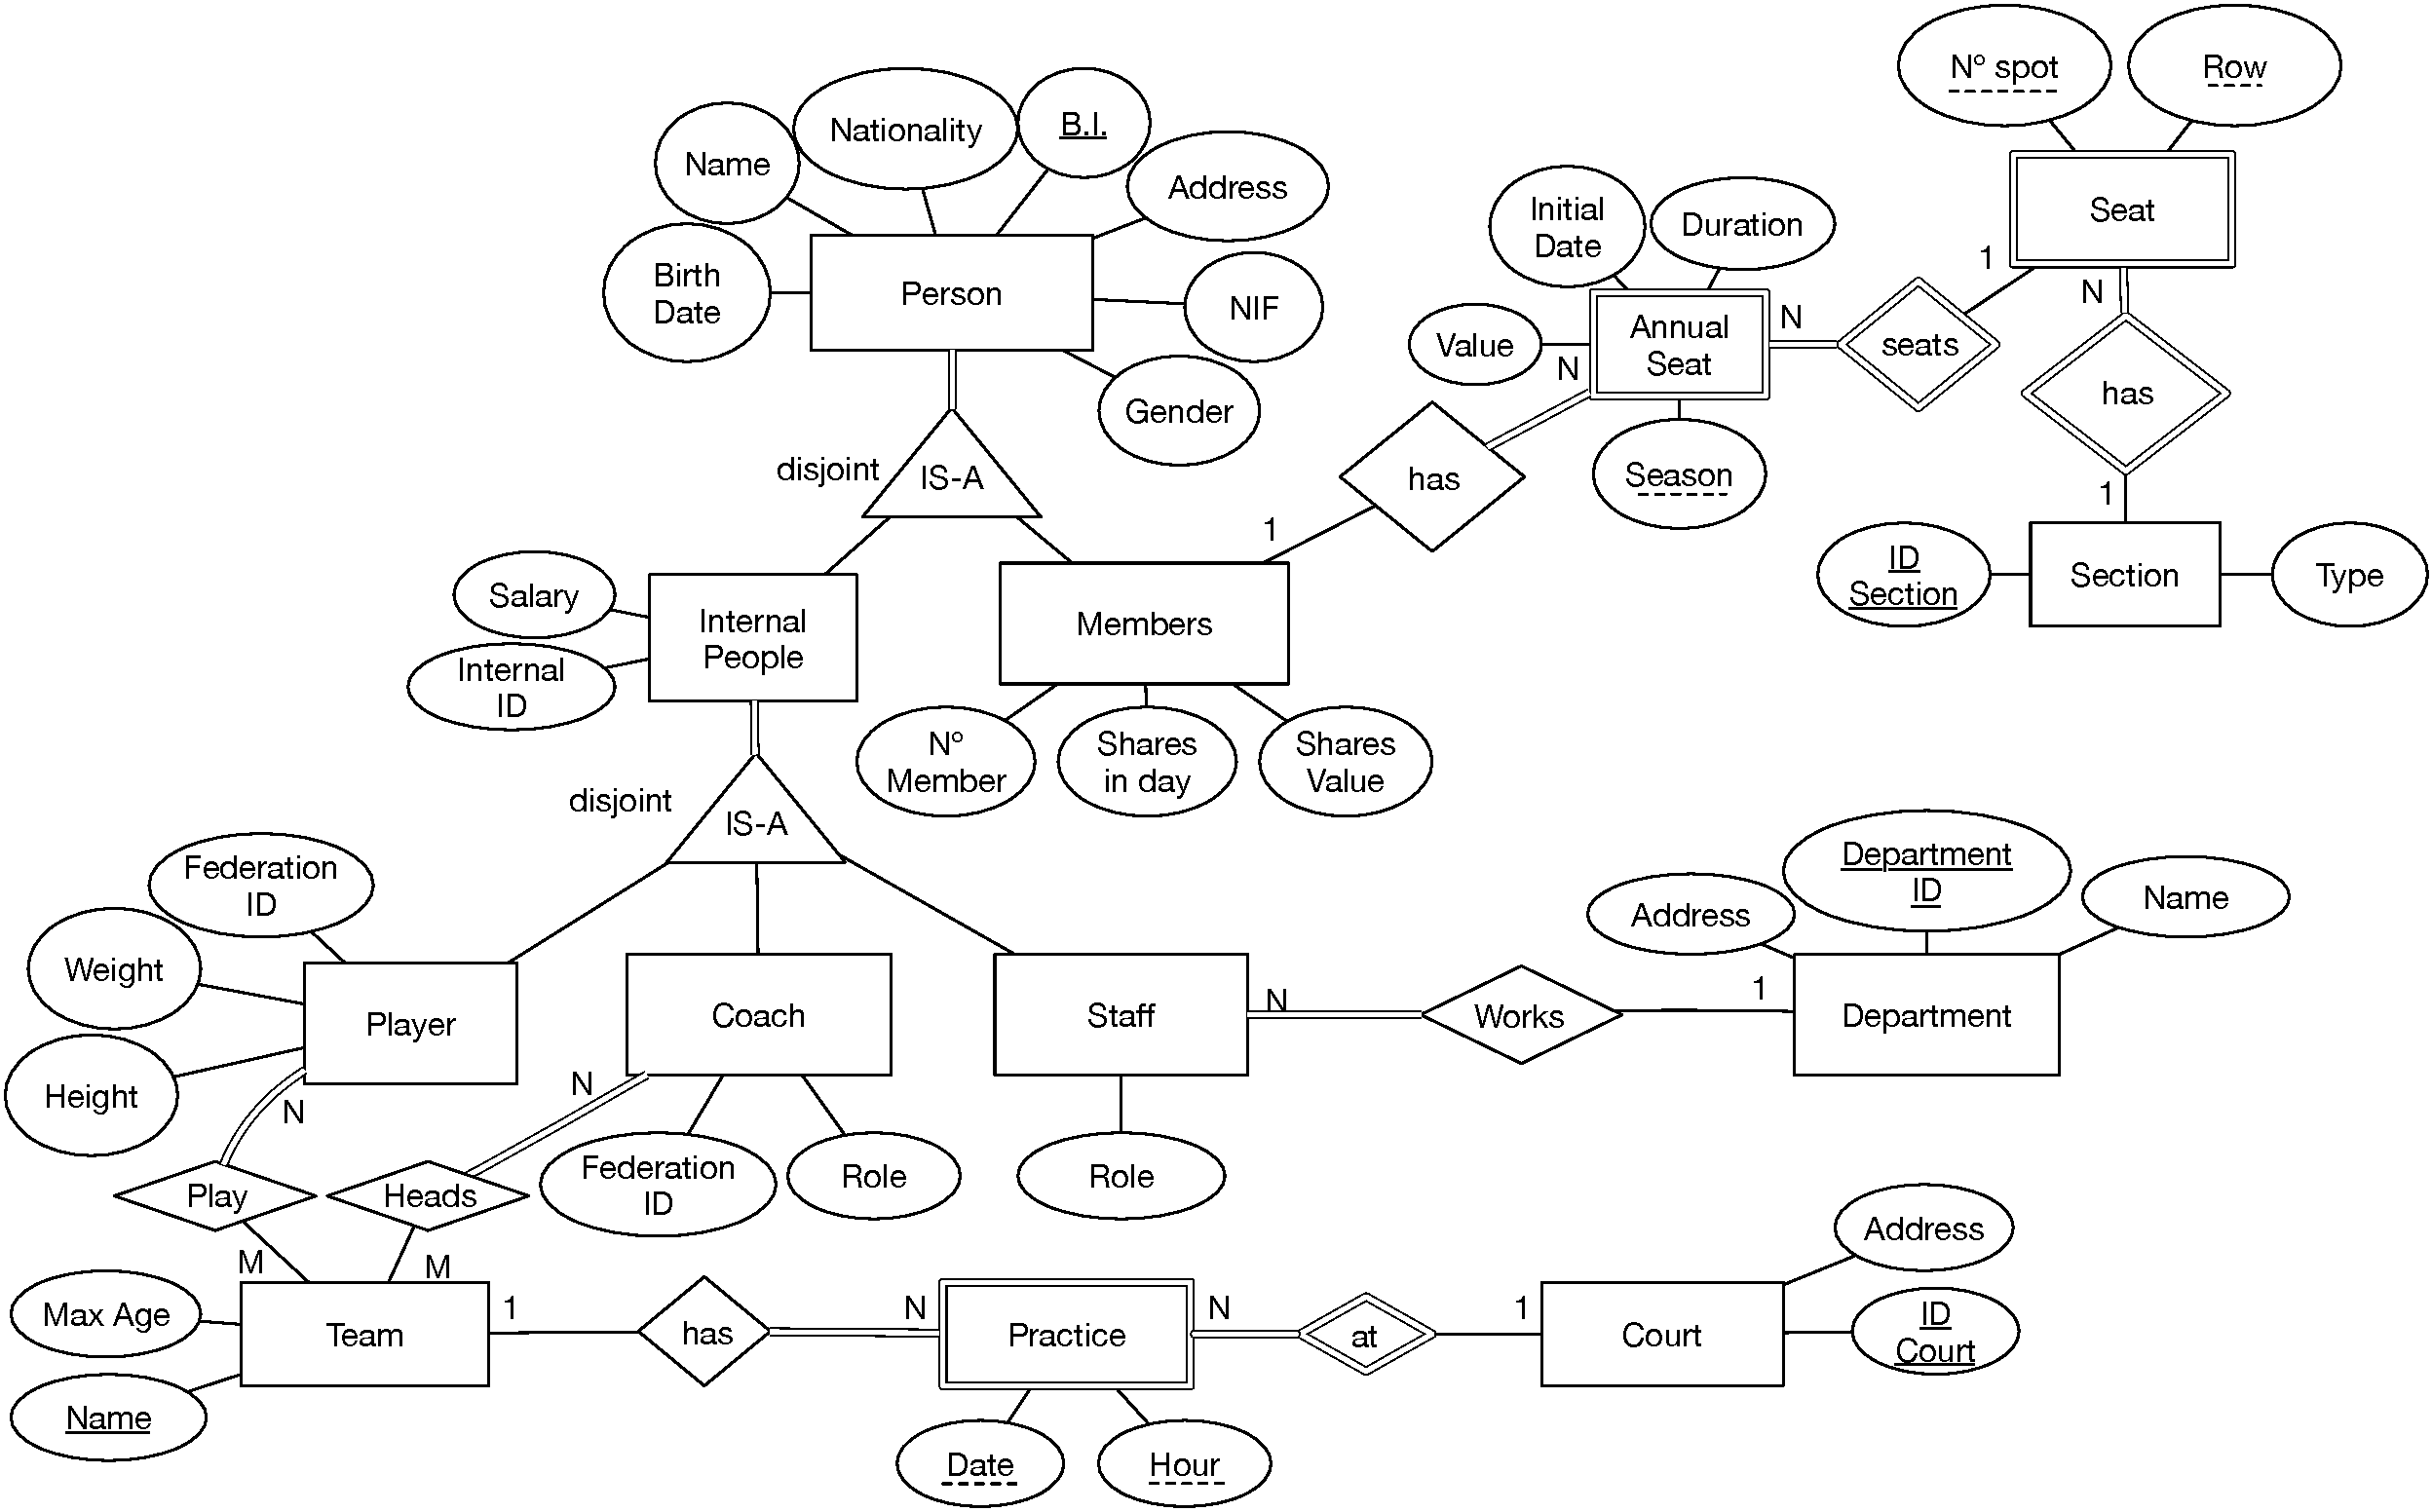
\includegraphics[width=135mm,scale=1]{EER.pdf}
 \caption{\\Diagrama entidade relação}\label{fig:eer}
\end{figure}

As entidades e os seus atributos correspondem à análise de requisitos realizada anteriormente. As relações são todas binárias.

\newpage
\section{Esquema Relacional da BD}
Após a construção do nosso desenho conceptual procedeu-se à elaboração do Modelo Relacional. Este modelo foi construído tendo por base o diagrama entidade relação e as regras para a realização desta tarefa. Cada entidade e cada relação irá gerar uma única tabela e após realizados os passos para conversão do desenho conceptual no modelo relacional 
foi criado o modelo relacional\ref{fig:mr}.

\begin{figure}[!htb]
 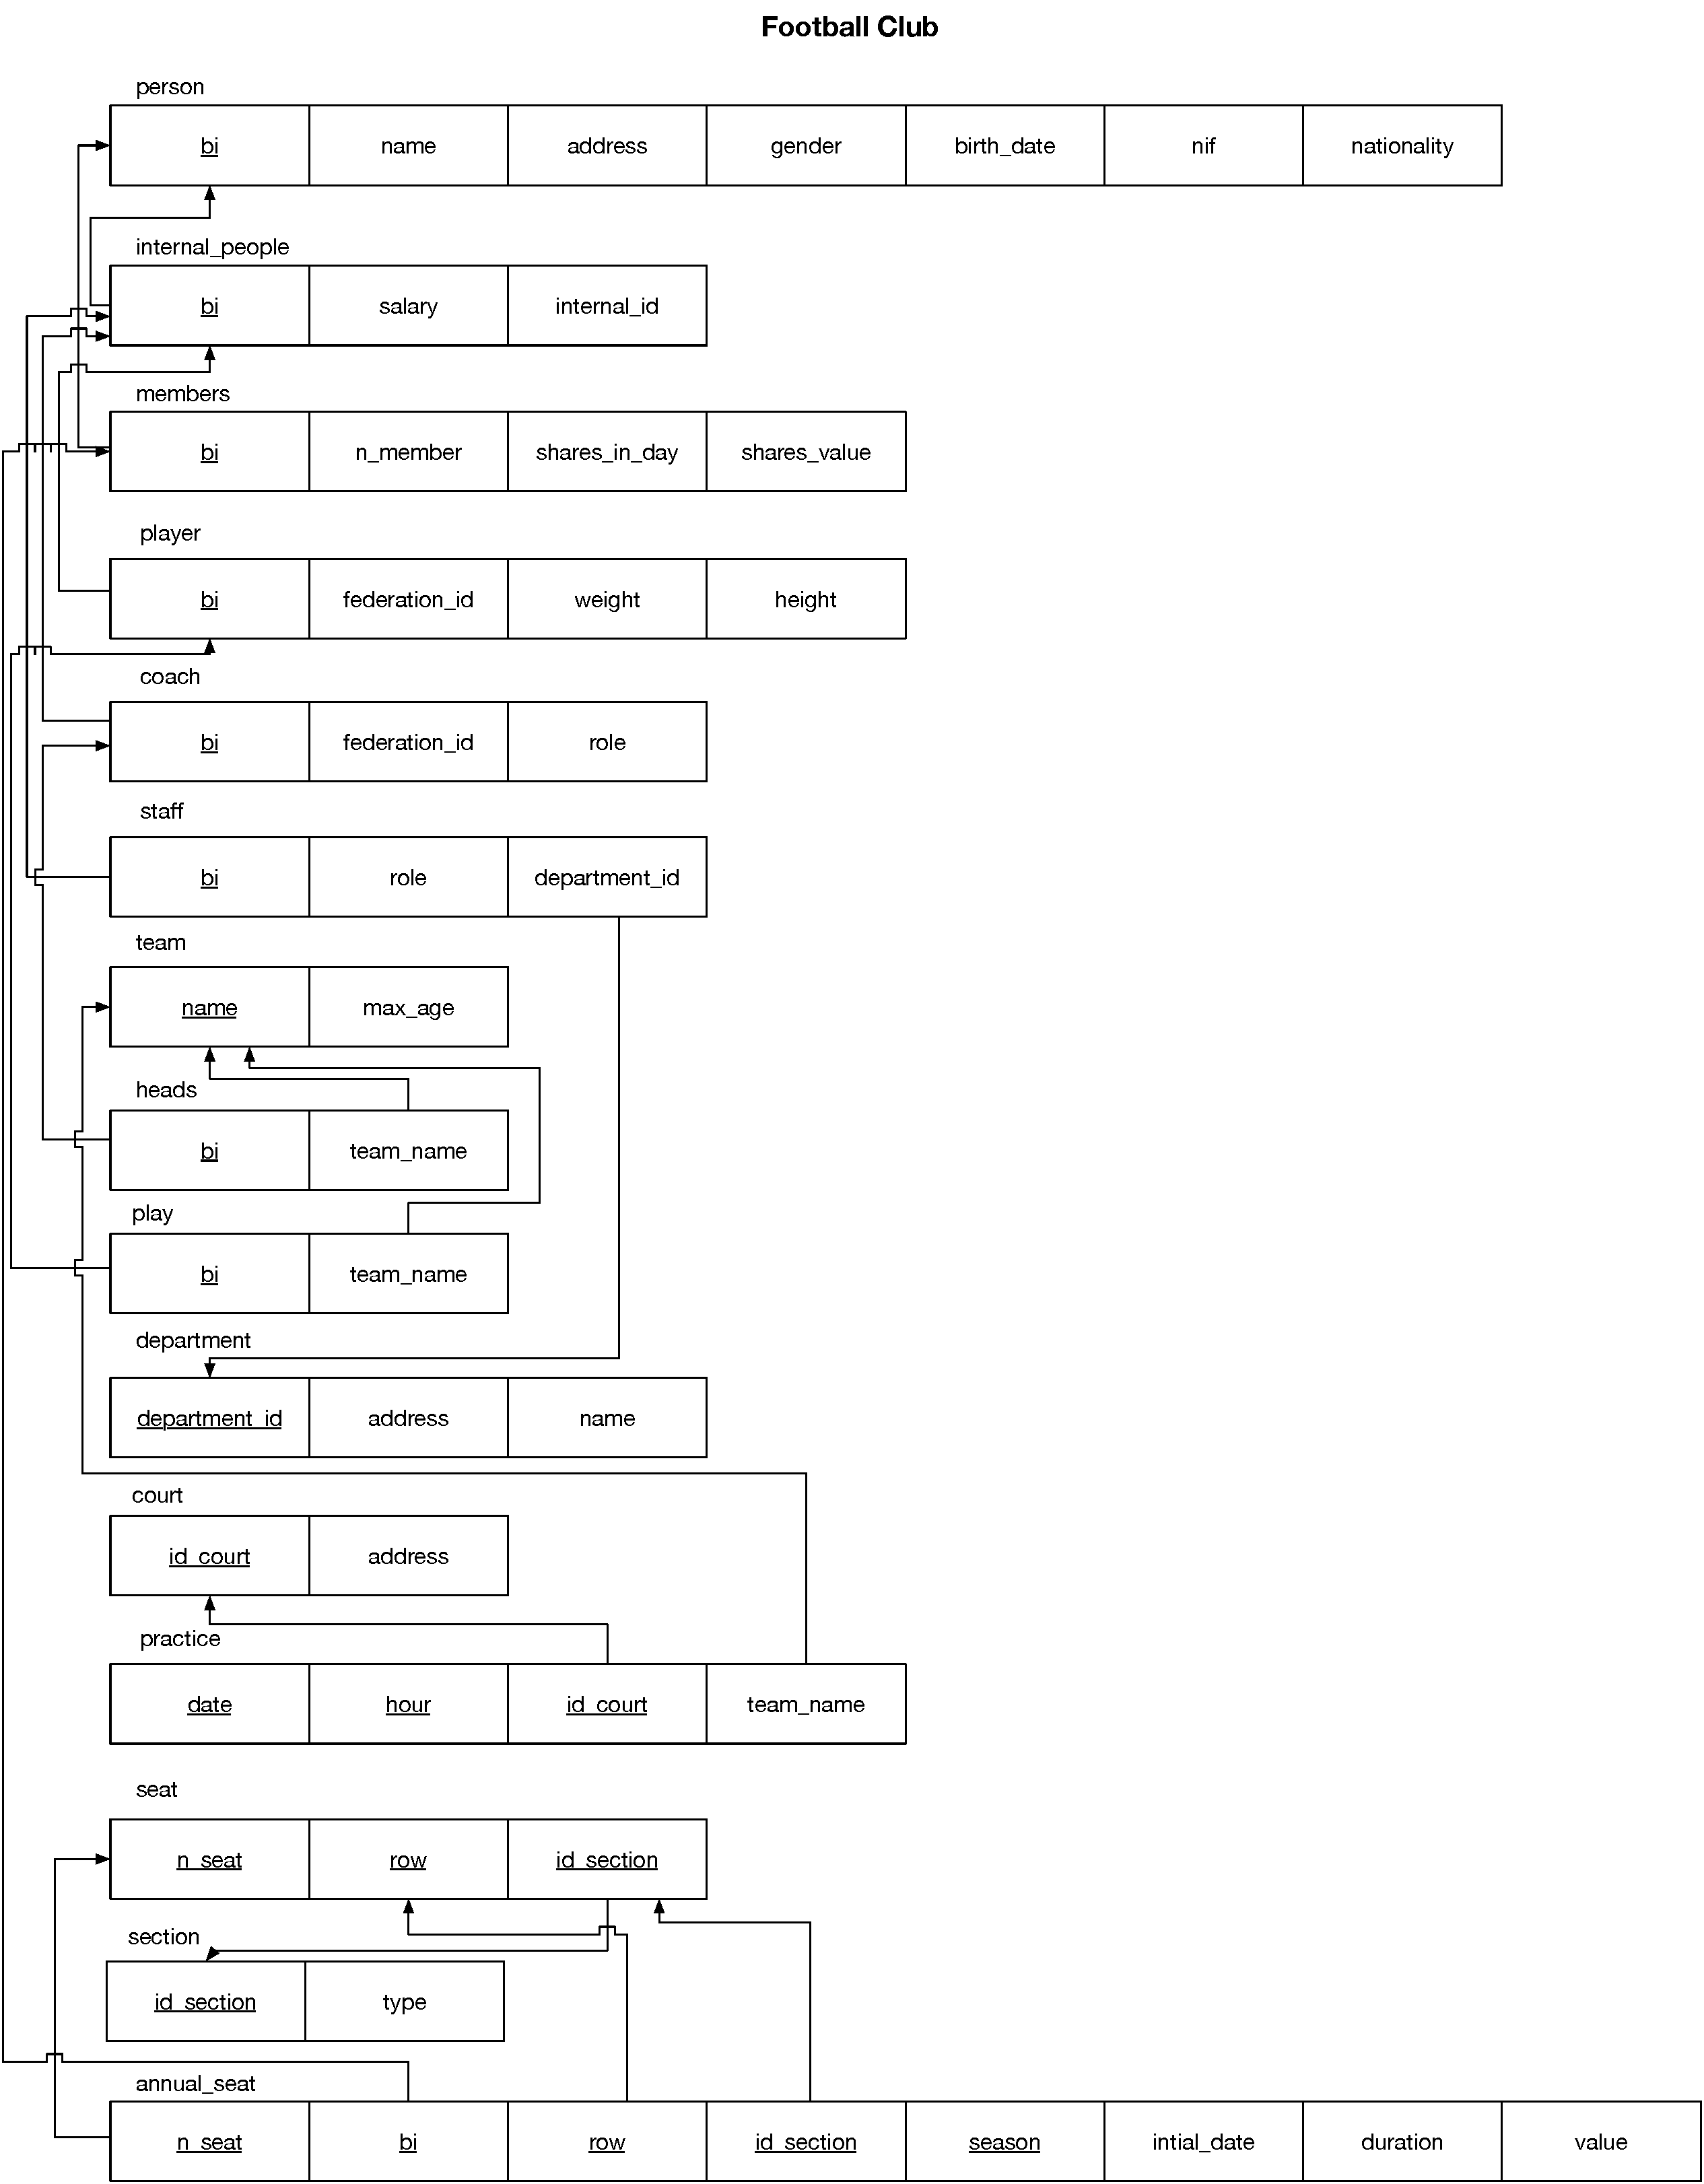
\includegraphics[width=115mm,scale=1]{modelo_relacional.pdf}
 \caption{\\Modelo relacional}\label{fig:mr}
\end{figure}

\newpage
\section{Normalização}
Para garantir a eficiência, a não existência de redundâncias e permitir a integridade referencial entre relações tive-se de usar normalizações.

Para realizar a normalização do nosso projeto teve-se em conta alguns conceitos. Inicialmente começa-se por garantir a 1FN, seguido da 2FN e usualmente terminando na 3FN. No entanto, em algumas situações a 3FN ainda apresenta algumas anomalias.
\\

Uma relação diz-se na 1FN quando:

- Os atributos são atómicos (simples e  indivisíveis), ou seja, não permite atributos composto ou multivalor.

- Não suporta relações dentro de relações, ou seja, não é possível utilizar uma relação como valor de um atributo de um tuplo.
\\

Uma relação diz-se na 2FN quando:

- Está na 1FN.

- Todos os atributos não pertencentes a qualquer chave candidata dependem totalmente da chave e não de parte dela.
\\

Uma relação diz-se na 3FN quando:

- Está na 2FN.

- Todos os atributos não chave não dependem funcionalmente uns dos outros, ou seja, são funcionalmente dependentes só e apenas da chave da relação.
\\

Uma relação diz-se na BCNF quando:

- Está na 3FN.

- Todos os atributos são funcionalmente dependentes da chave da relação, de toda a chave e de nada mais.
\\

Após a análise do nosso projecto pôde-se concluir que já se encontrava na 3FN pois não tem dependências transitivas e todos os atributos dependem da chave primária da sua relação.
\\

Como forma de demonstrar como foi realizada esta análise temos o seguinte exemplo:

\begin{figure}[!htb]
 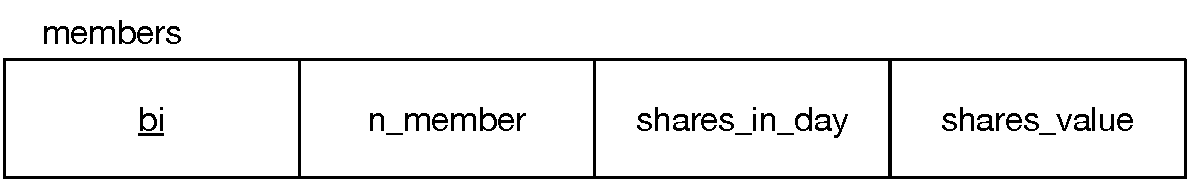
\includegraphics[width=40mm,scale=0.5]{exemplo_normalizacao.pdf}
\end{figure}

Neste exemplo temos a nossa relação Membro, que como pode-se verificar não existem atributos repetidos, multivalores ou compostos, estando assim na 1FN.

Esta relação também se encontra na 2FN, pois está na 1FN e todos os atributos dependem da chave primária da relação, ou seja, do BI.

Já está portanto na 3FN porque não tem dependências transitivas e todos os atributos dependem da chave primária.

\section{View's}
Foi decidido não usar views no desenvolvimento do nosso sistema. 

Em contra partida decidiu-se usar UDF's por estas serem mais seguras, serem compiladas e optimizadas, serem boas para ser utilizadas para incorporar lógica complexa dentro de uma consulta. 

As udf's também previnem a alteração ou remoção de objetos/tabelas utilizadas pela função.

Já as views não permitem esta camada de segurança, sendo assim, decidiu-se apenas usar UDF's para consulta de dados.

\newpage
\section{Índices}
Com o aumento do volume de dados, os pedidos de consulta começam a ter tempos de resposta maiores, pois os dados que existem nas tabelas encontram-se desorganizados. Para contrariar este aumento dos tempos de resposta devemos manter as tabelas organizadas de forma a que as consultas sejam efetuadas mais rapidamente. A utilização de índices nos campos que mais frequentemente serão utilizados é a maneira indicada, onde um ponteiro é criado para a posição real de cada registo.


Para tornar as nossas pesquisas mais eficientes introduzimos vários índices que achamos necessários (pesquisas feitas por dados não primários), do tipo NonClustered, pois os índices do tipo Clustered são automaticamente criados aquando da criação de uma tabela pois vai corresponder às chaves primárias.


Foram utilizados em todos os índices, um FILLFACTOR=75 com pad{\textunderscore}index, sendo que o primeiro determina a percentagem de espaço em cada página , quando um índice é criado, e o segundo, aplica às páginas de nível intermediário do índice a percentagem especificada pelo FILLFACTOR.
\\

Índice "indexactiveseat", exemplo:
\\

\begin{lstlisting}
go

CREATE NONCLUSTERED INDEX indexactiveseat ON football.seat(active)
WITH (FILLFACTOR=75,pad_index=ON);
\end{lstlisting}
 \vspace{0,5in}
Restantes índices estão disponíveis em anexo(ref):
\\


\newpage

\section{Stored Procedures}
Dicidiu-se usar stored procedures para criar uma camada de abstracção entre o modelo de dados, a sua manipulação e a camada aplicacional. A adopção desta abordagem permite-nos criar de forma segura, com boa performance e que garante a integridade dos dados, métodos para criar, modificar e apagar modelo de dados do nosso sistema de base de dados.

Outro dos motivos foi garantir um contrato de utilização entre o "developer" da aplicação e a utilização do nosso modelo de dados, permitindo assim especificar que parâmetros são necessários para realizar cada operação e garantindo também um bom controlo de erro avisando-o com T-SQL Raise Error quando este não estiver a cumprir o contrato.

As stored procedures ao contrário de um uso do nosso modelo de dados em DML permite que o conjunto de instruções compiladas na Stored Procedure  não tenham de ser recompiladas cada vez que o procedimento é invocado, sendo estas, apenas compiladas na primeira vez que são executadas e depois disso são guardadas em cache, sendo que isto permite maior rapidez no acesso ao modelo de dados.

Sendo assim, o principal foco em todas as stored procedures que se desenvolveu foi procurar garantir um bom controlo de erro para a camada aplicacional e que a criação, alteração ou remoção de dados do nosso modelo de dados fosse realizada de forma consistente.

De forma a garantir que as stored procedures responsáveis pela manipulação de dados em caso de erro na inserção de um grupo de instruções, os dados continuem consistentes  decidiu-se usar "Transactions".

\begin{lstlisting}
go 

CREATE PROCEDURE football.sp_createPlayer
  @bi				INT, 
  @name				VARCHAR(75),
  @address			VARCHAR(75), 
  @birth_date		DATE, 
  @nif				INT, 
  @gender			VARCHAR(1), 
  @nationality		VARCHAR(75),
  @salary			MONEY,
  @federation_id	INT,
  @weight			INT,
  @height			INT
WITH ENCRYPTION
AS 
	--Para garantir que todos os parametros enviados nao sao NULL decidiu-se garantir primeiro este contrato com um IF.
	 
	IF @bi is null OR @name is null OR @address is null OR @birth_date is null OR @nif is null OR 
		@gender is null OR @nationality is null OR @salary is null OR @federation_id is null OR
		@weight is null OR @height is null
	BEGIN
		-- Como este erro normalmente e causado pelo developer aplicacional optou-se por nao fazer um RAISE ERROR, contudo tambem poderia-se ter sido feito
		
		PRINT 'The bi, name, address, birth_date, nif, nationality, salary, federation_id, weight and height can not be null!'
		RETURN
	END
	
	DECLARE @count int

	-- Uma das restricoes no nosso modelo de dados e que nao podem existir pessoas com o mesmo BI, com este trexo de codigo garantimos isso e caso 
	-- check if the BI is already in use
	SELECT @count = count(bi) FROM football.person WHERE bi = @bi;

	IF @count != 0
	BEGIN
		RAISERROR ('The BI id is already in use!', 14, 1)
		RETURN
	END
		
	-- Nao faz sentido que um jogador e um treinador tenham o mesmo ID dentro da federacao, sendo assim tambem tem de ser comprido este contrato. Tambem se fez um Trigger para garantir este contrato num possivel manipulamento direto do modelo de dados
	
	-- check if the federation id is already in use
	SELECT @count = count(federation_id) FROM football.player WHERE federation_id = @federation_id;

	IF @count != 0
	BEGIN
		RAISERROR ('The federation id is already in use!', 14, 1)
		RETURN
	END
	
	-- check if the federation id is already in use
	SELECT @count = count(federation_id) FROM football.coach WHERE federation_id = @federation_id;

	IF @count != 0
	BEGIN
		RAISERROR ('The federation id is already in use by one coach!', 14, 1)
		RETURN
	END
	
	-- NIF e sempre unico
	
	-- check if the NIF is already in use
	SELECT @count = count(nif) FROM football.person WHERE nif = @nif;

	IF @count != 0
	BEGIN
		RAISERROR ('The NIF id is already in use!', 14, 1)
		RETURN
	END

	BEGIN TRANSACTION;
	
	--  Para garantir a integridade do nosso modelo de dados e necessario garantir que este conjunto de instrucoes sejam executadas e concluidas corretamente em conjunto e caso uma delas nao seja concluida com sucesso deve ser feito um RollBack garantindo assim que apenas serao inseridos dados de forma correta.
	
	BEGIN TRY
		INSERT INTO football.person 
					([bi], 
					 [name], 
					 [address], 
					 [birth_date], 
					 [nif], 
					 [gender],
					 [nationality]) 
		VALUES      ( @bi, 
					  @name, 
					  @address, 
					  @birth_date, 
					  @nif, 
					  @gender,
					  @nationality) 

		INSERT INTO football.internal_people 
					([bi], 
					 [salary]) 
		VALUES      ( @bi, 
					  @salary) 

		INSERT INTO football.player 
					([bi], 
					 [federation_id], 
					 [weight],
					 [height]) 
		VALUES      ( @bi, 
					  @federation_id, 
					  @weight,
					  @height)
		COMMIT TRANSACTION;
	END TRY
	BEGIN CATCH
		RAISERROR ('An error occurred when creating the player!', 14, 1)
		ROLLBACK TRANSACTION;
	END CATCH;

\end{lstlisting}
 \vspace{0,5in}

Restantes stored procedures estão disponíveis em anexo. (ref)

\newpage

\section{User-defined functions}
As UDF's no nosso modelo de dados desempenham o papel de vistas dado que não temos nenhuma "View". Uma user defined function representa várias vantagens em relação a uma view, podem ser usadas para incorporar lógica complexa numa pesquisa, podem aceitar parâmetros e usando schema binding previne a alteração ou remoção de objectos utilizados pela função.

Estas apresentam também a mesma característica do que os SPs por serem igualmente compilados e optimizados. Sendo assim o modelo de dados fica muito mais simples de ser usado e rápido.

Na maior parte das triggers optámos por uma lógica de quando os parâmetros de entrada fossem NULL a UDF retornaria todos os resultados da base de dados. Quando não fosse NULL ela retornaria resultados específicos.


\begin{lstlisting}
go

CREATE FUNCTION football.udf_players_data_grid(@team_name VARCHAR(50)=null)
RETURNS @table TABLE ("internal id" int, "bi" int, "name" varchar(75), "salary" money, "gender" varchar(1), "federation_id" int)
WITH SCHEMABINDING, ENCRYPTION
AS
BEGIN
	-- Quando @team_name e null mostra todos os jogadores de determinada equipa
	IF (@team_name is null)
		BEGIN
			INSERT @table SELECT	internal_people.internal_id AS 'internal id', person.bi, person.name, internal_people.salary, person.gender, player.federation_id AS 'federation id'
			FROM	(football.player JOIN (football.internal_people JOIN
football.person ON internal_people.bi = person.bi) ON player.bi = football.internal_people.bi);
		END;
		
	-- Quando @team_name nao e null entao mostra os detalhes de um jogador de determinada equipa
	ELSE
		BEGIN
			INSERT @table SELECT	internal_people.internal_id AS 'internal id', person.bi, person.name, internal_people.salary, person.gender, player.federation_id AS 'federation id'
			FROM	(football.play JOIN	(football.player JOIN (football.internal_people JOIN football.person ON internal_people.bi = person.bi) ON player.bi = football.internal_people.bi) ON play.bi = player.bi)
			WHERE team_name = @team_name;
		END;
	RETURN;
END;
\end{lstlisting}
 \vspace{0,5in}

Restantes user defined functions estão disponíveis em anexo. (ref)

\newpage
\section{Triggers}
De forma a garantir uma maior consistência e integridade da base de dados, foram utilizados alguns triggers. Estes são funções que são ativadas aquando de um insert, update ou delete numa determinada tabela de dados.

No nosso caso, foi criado, por exemplo, um  trigger que ocorre quando existe um pedido de delete na tabela "seat", este em vez de ser removido, altera o valor da variável "active" para 0 (INSTEAD OF).
O resto dos triggers utilizados resumem-se a verificações, no nosso caso, verificar se determinado "federation{\textunderscore}id" já existe aquando de um create ou de um update nas tabelas "coach" e "player".
Restantes triggers estão disponíveis em anexo(ref)
\\

\begin{lstlisting}
CREATE Trigger seatTrigger ON football.seat
INSTEAD OF DELETE
AS
	SET NOCOUNT ON;
	DECLARE @n_seat INT;
	DECLARE @row VARCHAR(1);
	DECLARE @id_Section INT;

	SELECT @n_seat = deleted.n_seat FROM deleted;
	SELECT @row = deleted.row FROM deleted;
	SELECT @id_section = deleted.id_section FROM deleted;
	
	-- Quando um pedido delete e executado na tabela football.seat, este trigger e ativado e em vez de apagar o "seat", altera a variavel "active" para o valor 0.
	
	BEGIN
		UPDATE football.seat SET
			   active = 0
			   WHERE seat.n_seat = @n_seat AND seat.row = @row AND seat.id_section = @id_section;
	END
\end{lstlisting}
 \vspace{0,5in}

\newpage
\section{Aplicação Utilizador}
A aplicação utilizador criada para este projecto, foi elaborada em conjunto com a disciplina de Interação Humano-Computador, em WPF/C\#.

Consiste num sistema de gestão de um clube de futebol, onde é possível efectuar as operações de inserção, alteração e remoção de entidades da Base de Dados, e ainda consultar estatísticas do clube.
\\

\begin{figure}[!htb]
 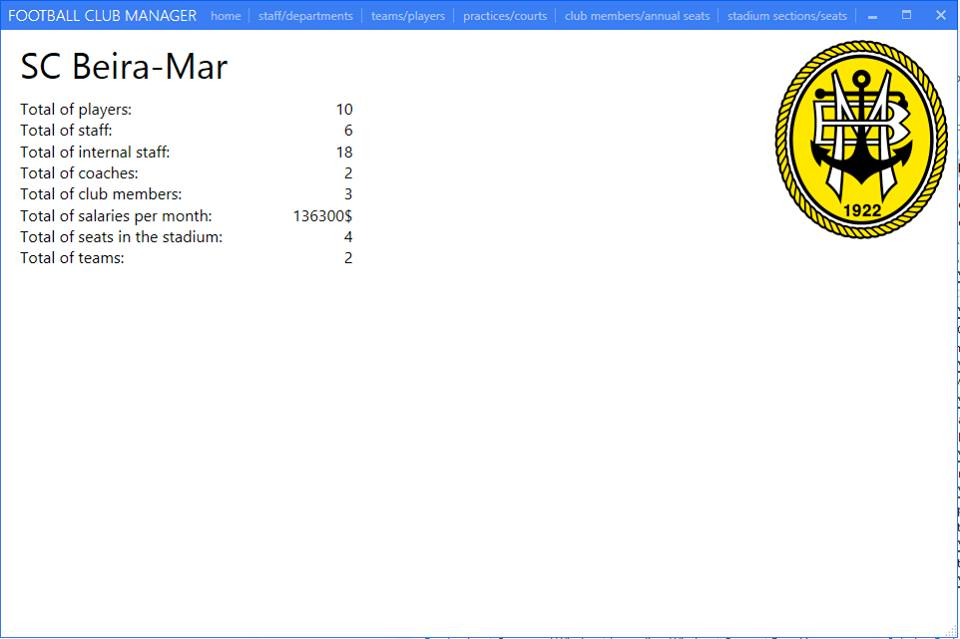
\includegraphics[width=135mm,scale=1]{app_home_page.jpg}
 \caption{\\Página Inicial}\label{fig:eer}
\end{figure}

\begin{figure}[!htb]
 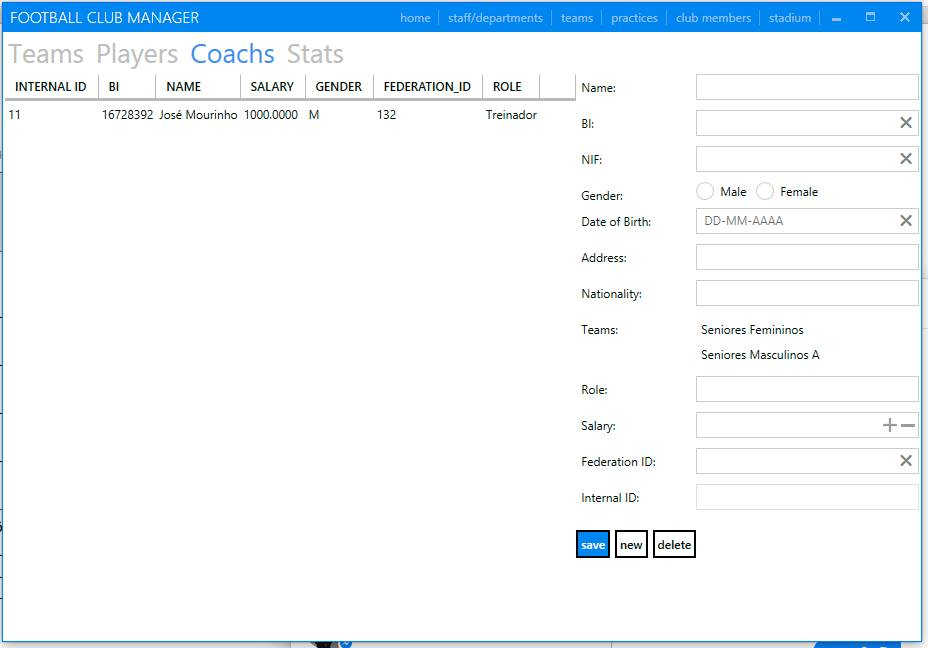
\includegraphics[width=135mm,scale=1]{app_add_coach.jpg}
 \caption{\\Página de listagem de Treinadores}\label{fig:eer}
\end{figure}


\clearpage
\section{Conclusão}
Os objectivos propostos foram alcançados, abordando grande parte dos conceitos leccionados na disciplina de Base de Dados, tanto na componente teórica como prática.
Foram efectuadas várias versões tanto do diagrama entidade-relação como do esquema relacional da Base de Dados, pois consoante se ia progredindo na elaboração do trabalho era necessário fazer alterações que se achassem necessárias.

Como foi referido neste relatório, a aplicação para o utilizador foi elaborada em conjunto com  a disciplina de Interação Humano-Computador, pelo que nos permitiu utilizar os conhecimentos adquiridos nesta mesma disciplina em WPF/C\#.

Concluindo, foi um trabalho bastante útil para o nosso desenvolvimento enquanto estudantes da área de Engenharia de Computadores e Telemática, pois permitiu a prática dos conceitos adquiridos na disciplina de Base de Dados.

\newpage
\section{Referências}

\begin{itemize}
	\item Mahapps - http://mahapps.com/ 
	\item Protection from SQL Injection http://programming-review.com/stop-mysql-injection/ 
	\item Data Grid selected http://blog.scottlogic.com/2008/12/02/wpf-datagrid-detecting-clicked-cell-and-row.html 
	\item Data Grid http://www.codeproject.com/Articles/30905/WPF-DataGrid-Practical-Examples\#displaying 
	\item Slides das aulas teóricas
\end{itemize}


\newpage
\section{Anexos}
\subsection*{Inserts}
annual{\textunderscore}seat.sql
\begin{lstlisting} 
-- use p4g5;
use p4g5;


INSERT INTO football.annual_seat (n_seat, row, id_section, start_date, duration, value, bi, season) VALUES (11, 'H', 2, '2014/09/02', 10, 95, 15672829, 2014);

\end{lstlisting}

coach.sql
\begin{lstlisting} 
-- use p4g5;
use p4g5;

--Seniores Masculinos

INSERT INTO football.coach(bi, federation_id, role) VALUES (16728392, 132, 'Treinador');

--Seniores Femininos
INSERT INTO football.coach (bi, federation_id, role) VALUES (49102019, 245, 'Treinador');
\end{lstlisting}

court.sql
\begin{lstlisting} 
-- use p4g5;
use p4g5;

INSERT INTO football.court(address) VALUES ('Cidade do Dragao');
INSERT INTO football.court(address) VALUES ('Cidade do Estadio');

\end{lstlisting}

department.sql
\begin{lstlisting} 
-- use p4g5;
use p4g5;

INSERT INTO football.department (address, name) VALUES ('Avenida do Dragao', 'Direccao');
INSERT INTO football.department (address, name) VALUES ('Rua do Estadio', 'Financeiro');
INSERT INTO football.department (address, name) VALUES ('Rua da Relva', 'Comercial');



\end{lstlisting}

heads.sql
\begin{lstlisting} 
-- use p4g5;
use p4g5;

--Seniores Masculinos

INSERT INTO football.heads(bi, team_name) VALUES (16728392, 'Seniores Masculinos');

--Seniores Femininos
INSERT INTO football.heads (bi, team_name) VALUES (49102019, 'Seniores Femininos');
\end{lstlisting}

internal{\textunderscore}people.sql
\begin{lstlisting} 
-- use p4g5;
use p4g5;

--Jogadores

INSERT INTO football.internal_people (bi, salary) VALUES (12345678, 50000);
INSERT INTO football.internal_people (bi, salary) VALUES (77777777, 10000);
INSERT INTO football.internal_people (bi, salary) VALUES (12445678, 0);
INSERT INTO football.internal_people (bi, salary) VALUES (39522123, 250);
INSERT INTO football.internal_people (bi, salary) VALUES (40128390, 50);
INSERT INTO football.internal_people (bi, salary) VALUES (52131283, 0);
INSERT INTO football.internal_people (bi, salary) VALUES (43123123, 0);
INSERT INTO football.internal_people (bi, salary) VALUES (12895726, 300);
INSERT INTO football.internal_people (bi, salary) VALUES (46728109, 0);
INSERT INTO football.internal_people (bi, salary) VALUES (90872134, 0);

--Treinadores

INSERT INTO football.internal_people (bi, salary) VALUES (16728392, 40000);
INSERT INTO football.internal_people (bi, salary) VALUES (49102019, 250);

--Staff

INSERT INTO football.internal_people (bi, salary) VALUES (13124523, 100);
INSERT INTO football.internal_people (bi, salary) VALUES (14563792, 1000);
INSERT INTO football.internal_people (bi, salary) VALUES (29675821, 1250);
INSERT INTO football.internal_people (bi, salary) VALUES (16758290, 30000);
INSERT INTO football.internal_people (bi, salary) VALUES (19283847, 850);
INSERT INTO football.internal_people (bi, salary) VALUES (39821392, 1500);

\end{lstlisting}

members.sql
\begin{lstlisting} 
-- use p4g5;
use p4g5;


--Sem Lugar Anual

INSERT INTO football.members(bi, shares_in_day, shares_value) VALUES (26718293, 2014, 20);
INSERT INTO football.members (bi, shares_in_day, shares_value) VALUES (28372192, 2015, 30);

--Com Lugar Anual

INSERT INTO football.members (bi, shares_in_day, shares_value) VALUES (15672829, 2015, 50);

\end{lstlisting}

person.sql
\begin{lstlisting} 
-- use p4g5;
use p4g5;

--Jogadores
INSERT INTO football.person (bi, name, address, birth_date, nif, gender, nationality) VALUES (12345678, 'Cristiano Ronaldo', 'Rua das bananas', '1985/02/05', 12345678, 'M', 'Portuguesa');
INSERT INTO football.person (bi, name, address, birth_date, nif, gender, nationality) VALUES (77777777, 'Ricardo Quaresma', 'Avenida do Dragao', '1983/09/26', 77777777, 'M', 'Portuguesa'); 
INSERT INTO football.person (bi, name, address, birth_date, nif, gender, nationality) VALUES (12445678, 'Pedro Costa', 'Rua das cavacas', '1995/06/05', 12344678, 'M', 'Portuguesa'); 
INSERT INTO football.person (bi, name, address, birth_date, nif, gender, nationality) VALUES (39522123, 'Eduardo Santos', 'Travessa do Rio', '1990/02/25', 15326722, 'M', 'Portuguesa'); 
INSERT INTO football.person (bi, name, address, birth_date, nif, gender, nationality) VALUES (40128390, 'Bernardo Pires', 'Avenida Principal', '1997/02/16', 22146758, 'M', 'Portuguesa'); 
INSERT INTO football.person (bi, name, address, birth_date, nif, gender, nationality) VALUES (52131283, 'Rita Marques', 'Travessa do Rossio', '1997/01/02', 21321421, 'F', 'Portuguesa');
INSERT INTO football.person (bi, name, address, birth_date, nif, gender, nationality) VALUES (43123123, 'Luisa Norte', 'Rua da fonte', '1990/07/06', 23113123, 'F', 'Portuguesa'); 
INSERT INTO football.person (bi, name, address, birth_date, nif, gender, nationality) VALUES (12895726, 'Manuel Flores', 'Avenida do Bom-Samaritano', '1981/09/16', 12349882, 'M', 'Portuguesa');
INSERT INTO football.person (bi, name, address, birth_date, nif, gender, nationality) VALUES (46728109, 'Miguel Oliveira', 'Avenida do Paraiso', '1993/01/18', 32138211, 'M', 'Portuguesa');
INSERT INTO football.person (bi, name, address, birth_date, nif, gender, nationality) VALUES (90872134, 'Mara Luis', 'Rua da marisqueira', '1995/01/13', 67526192, 'F', 'Portuguesa'); 

--Treinadores

INSERT INTO football.person (bi, name, address, birth_date, nif, gender, nationality) VALUES (16728392, 'Jos Mourinho', 'Avenida de Inglaterra', '1965/08/05', 12324940, 'M', 'Portuguesa');
INSERT INTO football.person (bi, name, address, birth_date, nif, gender, nationality) VALUES (49102019, 'Carlos Ferreira', 'Rua da praia', '1977/01/30', 21837329, 'M', 'Portuguesa'); 

--Staff

INSERT INTO football.person (bi, name, address, birth_date, nif, gender, nationality) VALUES (13124523, 'Luis Pais', 'Rua Padre Xavier', '1965/08/29', 14052123, 'M', 'Portuguesa'); 
INSERT INTO football.person (bi, name, address, birth_date, nif, gender, nationality) VALUES (14563792, 'Maria Campos', 'Travessa das Camlias', '1977/09/06', 34520921, 'F', 'Portuguesa');
INSERT INTO football.person (bi, name, address, birth_date, nif, gender, nationality) VALUES (29675821, 'Eduarda Olivais', 'Rua das Bolas', '1965/01/20', 23156782, 'F', 'Portuguesa'); 
INSERT INTO football.person (bi, name, address, birth_date, nif, gender, nationality) VALUES (16758290, 'Jorge Nuno Pinto da Costa', 'Avenida do Dragao', '1937/12/28', 02134123, 'M', 'Portuguesa'); 
INSERT INTO football.person (bi, name, address, birth_date, nif, gender, nationality) VALUES (19283847, 'Pedro Paulo', 'Avenida do Doutor Luis', '1965/09/10', 47282910, 'M', 'Portuguesa');
INSERT INTO football.person (bi, name, address, birth_date, nif, gender, nationality) VALUES (39821392, 'Fernanda Pascoal', 'Rua de Maio', '1965/06/01', 21238291, 'F', 'Portuguesa');

--Socios

INSERT INTO football.person (bi, name, address, birth_date, nif, gender, nationality) VALUES (15672829, 'Jorge Jesus', 'Rua de Benfica', '1956/01/01', 21324124, 'M', 'Portuguesa'); 
INSERT INTO football.person (bi, name, address, birth_date, nif, gender, nationality) VALUES (26718293, 'Luis Simoes', 'Avenida do Macaco', '1993/11/22', 12383492, 'M', 'Portuguesa'); 
INSERT INTO football.person (bi, name, address, birth_date, nif, gender, nationality) VALUES (28372192, 'Rafael Luis', 'Avenida do Caloteiro', '1973/12/22', 32142422, 'M', 'Portuguesa');





\end{lstlisting}

play.sql
\begin{lstlisting} 
-- use p4g5;
use p4g5;

--Seniores Femininos

INSERT INTO football.play (bi, team_name) VALUES (52131283, 'Seniores Femininos');
INSERT INTO football.play (bi, team_name) VALUES (43123123, 'Seniores Femininos');
INSERT INTO football.play (bi, team_name) VALUES (90872134, 'Seniores Femininos');

--Seniores Masculinos

INSERT INTO football.play (bi, team_name) VALUES (12345678, 'Seniores Masculinos');
INSERT INTO football.play (bi, team_name) VALUES (77777777, 'Seniores Masculinos');
INSERT INTO football.play (bi, team_name) VALUES (12445678, 'Seniores Masculinos');
INSERT INTO football.play (bi, team_name) VALUES (39522123, 'Seniores Masculinos');
INSERT INTO football.play (bi, team_name) VALUES (40128390, 'Seniores Masculinos');
INSERT INTO football.play (bi, team_name) VALUES (12895726, 'Seniores Masculinos');
INSERT INTO football.play (bi, team_name) VALUES (46728109, 'Seniores Masculinos');
\end{lstlisting}

player.sql
\begin{lstlisting} 
-- use p4g5;
use p4g5;


--Seniores Femininos

INSERT INTO football.player (bi, federation_id, weight, height) VALUES (52131283, 1234, 59, 160);
INSERT INTO football.player (bi, federation_id, weight, height) VALUES (43123123, 09382, 58, 170);
INSERT INTO football.player (bi, federation_id, weight, height) VALUES (90872134, 23234, 52, 162);

--Seniores Masculinos

INSERT INTO football.player(bi, federation_id, weight, height) VALUES (12345678, 201, 77, 189);
INSERT INTO football.player (bi, federation_id, weight, height) VALUES (77777777, 30012, 75, 182);
INSERT INTO football.player (bi, federation_id, weight, height) VALUES (12445678, 2001, 70, 177);
INSERT INTO football.player (bi, federation_id, weight, height) VALUES (39522123, 3482, 72, 175);
INSERT INTO football.player (bi, federation_id, weight, height) VALUES (40128390, 1859, 69, 167);
INSERT INTO football.player (bi, federation_id, weight, height) VALUES (12895726, 2394, 80, 192);
INSERT INTO football.player (bi, federation_id, weight, height) VALUES (46728109, 19283, 82, 184);




\end{lstlisting}

practices.sql
\begin{lstlisting} 
-- use p4g5;
use p4g5;

INSERT INTO football.practice(date, hour, id_court, team_name) VALUES ('2015/05/21', '21:00', 1, 'Seniores Masculinos');
INSERT INTO football.practice(date, hour, id_court, team_name) VALUES ('2015/05/22', '19:00', 2, 'Seniores Femininos');
\end{lstlisting}

seat.sql
\begin{lstlisting} 
-- use p4g5;
use p4g5;

--Topo Norte

INSERT INTO football.seat(n_seat, row, id_section) VALUES (10, 'B', 1);
INSERT INTO football.seat(n_seat, row, id_section) VALUES (17, 'C', 1);

--Central

INSERT INTO football.seat(n_seat, row, id_section) VALUES (11, 'H', 2);
INSERT INTO football.seat(n_seat, row, id_section) VALUES (2, 'I', 2);
\end{lstlisting}

section.sql
\begin{lstlisting} 
-- use p4g5;
use p4g5;


INSERT INTO football.section(type) VALUES ('Topo Norte');
INSERT INTO football.section(type) VALUES ('Central');
\end{lstlisting}

staff.sql
\begin{lstlisting} 
-- use p4g5;
use p4g5;


--Direccao

INSERT INTO football.staff (bi, role, department_id) VALUES (16758290, 'Presidente', 1);
INSERT INTO football.staff (bi, role, department_id) VALUES (13124523, 'Vice-Presidente', 1);

--Departamento Financeiro

INSERT INTO football.staff (bi, role, department_id) VALUES (19283847, 'Director Financeiro', 2);
INSERT INTO football.staff (bi, role, department_id) VALUES (14563792, 'Gestor Financeiro', 2);

--Departamento Comercial

INSERT INTO football.staff (bi, role, department_id) VALUES (29675821, 'Director de Vendas', 3);
INSERT INTO football.staff (bi, role, department_id) VALUES (39821392, 'Vendedor', 3);


\end{lstlisting}

tables.sql
\begin{lstlisting} 
-- CREATE SCHEMA football;
use p4g5;

-- person
CREATE TABLE football.person(
    bi INT PRIMARY KEY CHECK(bi>0),
    name VARCHAR(75) NOT NULL,
    address VARCHAR(75) NOT NULL,
    birth_date DATE NOT NULL,
    nif INT UNIQUE NOT NULL,
	gender VARCHAR(1) NOT NULL CHECK (gender IN('M','F')),
	nationality VARCHAR(75) NOT NULL
);

-- internal people
CREATE TABLE football.internal_people(
    bi INT PRIMARY KEY,
    salary MONEY NOT NULL CHECK (salary >= 0),
    internal_id INT UNIQUE NOT NULL IDENTITY
);

-- ALTERs internal people
ALTER TABLE football.internal_people ADD CONSTRAINT FORPIBIPBI
FOREIGN KEY (bi) REFERENCES football.person(bi)
ON UPDATE CASCADE;

-- members
CREATE TABLE football.members(
    bi INT PRIMARY KEY,
    n_member INT NOT NULL UNIQUE IDENTITY,
    shares_in_day INT NOT NULL,
    shares_value MONEY NOT NULL CHECK (shares_value >= 0),
);

-- ALTERs members
ALTER TABLE football.members ADD CONSTRAINT FORSBIPBI
FOREIGN KEY (bi) REFERENCES football.person(bi)
ON UPDATE CASCADE;

-- player
CREATE TABLE football.player(
    bi INT PRIMARY KEY,
    federation_id INT UNIQUE NOT NULL CHECK(federation_id >= 0),
    weight int NOT NULL CHECK(weight > 0),
    height int NOT NULL CHECK(height > 0)
);

-- player ALTERs
ALTER TABLE football.player ADD CONSTRAINT FORJBIPIBI
FOREIGN KEY (bi) REFERENCES football.internal_people(bi)
ON UPDATE CASCADE;

-- coach
CREATE TABLE football.coach(
    bi INT PRIMARY KEY,
    federation_id INT NOT NULL CHECK(federation_id >= 0),
    role VARCHAR(50) NOT NULL
);

-- coach ALTERs
ALTER TABLE football.coach ADD CONSTRAINT FORTBIPIBI
FOREIGN KEY (bi) REFERENCES football.internal_people(bi)
ON UPDATE CASCADE;

-- STAFF CLUBE
CREATE TABLE football.staff(
    bi INT PRIMARY KEY,
    role VARCHAR(50) NOT NULL,
    department_id INT NOT NULL
);

-- STAFF ALTERs
ALTER TABLE football.staff ADD CONSTRAINT FORSCBIPIBI
FOREIGN KEY (bi) REFERENCES football.internal_people(bi)
ON UPDATE CASCADE;

-- department
CREATE TABLE football.department(
    department_id INT PRIMARY KEY IDENTITY,
    address VARCHAR(75) NOT NULL,
    name VARCHAR(75) NOT NULL
);

-- STAFF ALTERs
ALTER TABLE football.staff ADD CONSTRAINT FORSCIDDID
FOREIGN KEY (department_id) REFERENCES football.department(department_id)
ON UPDATE CASCADE;

-- ESCALAO
CREATE TABLE football.team(
    name VARCHAR(50) PRIMARY KEY,
    max_age INT NOT NULL CHECK(max_age > 0)
);

-- play
CREATE TABLE football.play(
    bi INT,
    team_name VARCHAR(50),
	PRIMARY KEY(bi, team_name)
);

-- ALTER play
ALTER TABLE football.play ADD CONSTRAINT FORJBIJBI
FOREIGN KEY (bi) REFERENCES football.player(bi)
ON UPDATE CASCADE;

ALTER TABLE football.play ADD CONSTRAINT FORJEEE
FOREIGN KEY (team_name) REFERENCES football.team(name)
ON UPDATE CASCADE;

-- heads
CREATE TABLE football.heads(
    bi int,
    team_name VARCHAR(50),
	PRIMARY KEY(bi, team_name)
);

-- ALTER heads
ALTER TABLE football.heads ADD CONSTRAINT FORDBITBI
FOREIGN KEY (bi) REFERENCES football.coach(bi)
ON UPDATE CASCADE;

ALTER TABLE football.heads ADD CONSTRAINT FORDEEE
FOREIGN KEY (team_name) REFERENCES football.team(name)
ON UPDATE CASCADE;

-- court
CREATE TABLE football.court(
    id_court INT PRIMARY KEY IDENTITY,
    address VARCHAR(150) NOT NULL
);

-- practice
CREATE TABLE football.practice(
    date DATE NOT NULL,
    hour TIME NOT NULL,
    id_court INT NOT NULL,
    team_name VARCHAR(50) NOT NULL,
    PRIMARY KEY(date, hour, id_court)
);

-- ALTERs practice
ALTER TABLE football.practice ADD CONSTRAINT FORTICCIC
FOREIGN KEY (id_court) REFERENCES football.court(id_court)
ON UPDATE CASCADE;

ALTER TABLE football.practice ADD CONSTRAINT FORTNEEN
FOREIGN KEY (team_name) REFERENCES football.team(name)
ON UPDATE CASCADE;

-- section
CREATE TABLE football.section(
    id_section INT PRIMARY KEY IDENTITY,
    type VARCHAR(50)
);

-- seat
CREATE TABLE football.seat(
    n_seat INT NOT NULL,
    row VARCHAR(1) NOT NULL,
    id_section INT NOT NULL,
    PRIMARY KEY(n_seat, row, id_section)
);

-- ALTER seat
ALTER TABLE football.seat ADD active BIT DEFAULT 1
ALTER TABLE football.seat ADD CONSTRAINT FORLISSIS
FOREIGN KEY (id_section)  REFERENCES football.section(id_section)
ON UPDATE CASCADE;

-- annual_seat
CREATE TABLE football.annual_seat(
  n_seat INT NOT NULL,
  row VARCHAR(1) NOT NULL,
  id_section INT NOT NULL,
  start_date DATE NOT NULL,
  duration INT NOT NULL,
  value INT NOT NULL,
  bi INT NOT NULL,
  season INT NOT NULL,
  PRIMARY KEY(n_seat, bi, row, id_section, season)
);



-- annual_seat ALTER's
ALTER TABLE football.annual_seat ADD CONSTRAINT FORLAL
FOREIGN KEY (n_seat, row, id_section) REFERENCES football.seat(n_seat, row, id_section)
ON UPDATE CASCADE;

ALTER TABLE football.annual_seat ADD CONSTRAINT FORLABISBI
FOREIGN KEY (bi) REFERENCES football.members(bi)
ON UPDATE CASCADE;

\end{lstlisting}

team.sql
\begin{lstlisting} 
-- use p4g5;
use p4g5;

INSERT INTO football.team(name, max_age) VALUES ('Seniores Masculinos', 50);
INSERT INTO football.team(name, max_age) VALUES ('Seniores Femininos', 50);

\end{lstlisting}

\newpage
\subsection*{Indexes}
seat.sql
\begin{lstlisting} 
use p4g5;

go

CREATE NONCLUSTERED INDEX indexactiveseat ON football.seat(active)
WITH (FILLFACTOR=75,pad_index=ON);

\end{lstlisting}

teams.sql
\begin{lstlisting} 
use p4g5;

go

CREATE NONCLUSTERED INDEX indexsalaryinternalpeople ON football.internal_people(salary)
WITH (FILLFACTOR=75,pad_index=ON);

go

CREATE NONCLUSTERED INDEX indexheightplayer ON football.player(height)
WITH (FILLFACTOR=75,pad_index=ON);

go

CREATE NONCLUSTERED INDEX indexweigthplayer ON football.player(weight)
WITH (FILLFACTOR=75,pad_index=ON);
\end{lstlisting}

\newpage
\subsection*{Store procedures}
annualSeat.sql
\begin{lstlisting} 
use p4g5;

go 

-- DROP PROC football.sp_createAnnualSeat

CREATE PROCEDURE football.sp_createAnnualSeat
  @bi				INT,  
  @start_date		DATE, 
  @n_seat			INT, 
  @row  			VARCHAR(1), 
  @value			INT,
  @id_section       INT,
  @season	        INT,
  @duration			INT

WITH ENCRYPTION
AS 
	IF @bi is null OR @start_date is null OR @n_seat is null OR @row is null OR @value is null OR 
		@id_section is null OR @season is null OR @duration is null
	BEGIN
		PRINT 'The bi, start_date, n_seat, row, value, id_section, season and duration can not be null!'
		RETURN
	END
	
	DECLARE @count int

	-- check if the BI exists
	SELECT @count = count(bi) FROM football.person WHERE bi = @bi;

	IF @count = 0
	BEGIN
		RAISERROR ('The BI that you provided do not exists!', 14, 1)
		RETURN
	END

	-- check if the Annual seat is already in use
	SELECT @count = count(bi) FROM football.annual_seat WHERE n_seat = @n_seat AND row = @row AND bi = @bi AND id_section = @id_section AND season = @season;

	IF @count != 0
	BEGIN
		RAISERROR ('The Annual seat is already in use!', 14, 1)
		RETURN
	END

	-- check if the Annual seat is already in use
	SELECT @count = count(n_seat) FROM football.annual_seat WHERE n_seat = @n_seat AND row = @row AND id_section = @id_section AND season = @season;

	IF @count != 0
	BEGIN
		RAISERROR ('The Annual seat is already in use!', 14, 1)
		RETURN
	END


	-- check if the seat exists
	SELECT @count = count(n_seat) FROM football.seat WHERE n_seat = @n_seat AND row = @row AND id_section = @id_section;

	IF @count = 0
	BEGIN
		RAISERROR ('The seat doesnt exist!', 14, 1)
		RETURN
	END

	BEGIN TRY
		INSERT INTO football.annual_seat 
					([n_seat], 
					 [row], 
					 [id_section], 
					 [start_date], 
					 [duration], 
					 [value],
					 [bi],
					 [season]) 
		VALUES      ( @n_seat, 
					  @row, 
					  @id_section, 
					  @start_date, 
					  @duration, 
					  @value,
					  @bi,
					  @season)
	END TRY
	BEGIN CATCH
		RAISERROR ('An error occurred when creating the annual seat!', 14, 1)
	END CATCH;


go 

-- DROP PROC football.sp_modifyAnnualSeat

CREATE PROCEDURE football.sp_modifyAnnualSeat
  @bi				INT,  
  @start_date		DATE, 
  @n_seat			INT, 
  @row  			VARCHAR(1), 
  @value			INT,
  @id_section       INT,
  @season	        INT,
  @duration			INT

WITH ENCRYPTION
AS 
	IF @bi is null OR @start_date is null OR @n_seat is null OR @row is null OR @value is null OR 
		@id_section is null OR @season is null OR @duration is null
	BEGIN
		PRINT 'The bi, start_date, n_seat, row, value, id_section, season and duration can not be null!'
		RETURN
	END
	
	DECLARE @count int

	-- check if the BI exists
	SELECT @count = count(bi) FROM football.person WHERE bi = @bi;

	IF @count = 0
	BEGIN
		RAISERROR ('The BI that you provided do not exists!', 14, 1)
		RETURN
	END

	-- check if the seat exists
	SELECT @count = count(n_seat) FROM football.seat WHERE n_seat = @n_seat AND row = @row AND id_section = @id_section;

	IF @count = 0
	BEGIN
		RAISERROR ('The seat doesnt exist!', 14, 1)
		RETURN
	END

	BEGIN TRY
		UPDATE  football.annual_seat SET
				start_date = @start_date,
				id_section = @id_section,
				duration = @duration,
				value = @value
		WHERE n_seat = @n_seat AND row = @row AND id_section = @id_section AND bi = @bi AND season = @season;
	END TRY
	BEGIN CATCH
		RAISERROR ('An error occurred when updating the annual seat!', 14, 1)
	END CATCH;

go 

-- DROP PROC football.sp_deleteAnnualSeat

CREATE PROCEDURE football.sp_deleteAnnualSeat
  @n_seat				INT,
  @row					VARCHAR(1),
  @id_section			INT,
  @bi					INT,
  @season				INT
WITH ENCRYPTION
AS 
	IF @bi is null OR @n_seat is null OR @id_section is null OR @row is null OR @season is null
	BEGIN
		PRINT 'The bi, n_seat, id_section, row and season can not be null!'
		RETURN
	END

	BEGIN TRY
		DELETE FROM football.annual_seat WHERE bi = @bi AND n_seat = @n_seat AND id_section = @id_section AND row = @row AND season = @season;
	END TRY
	BEGIN CATCH
		RAISERROR ('An error occurred when try delete the annual seat!', 14, 1)
	END CATCH;
\end{lstlisting}

coachs.sql
\begin{lstlisting} 
use p4g5;

go 

-- DROP PROC football.sp_createCoach

CREATE PROCEDURE football.sp_createCoach
  @bi				INT, 
  @name				VARCHAR(75),
  @address			VARCHAR(75), 
  @birth_date		DATE, 
  @nif				INT, 
  @gender			VARCHAR(1), 
  @nationality		VARCHAR(75),
  @salary			MONEY,
  @federation_id	INT,
  @role				VARCHAR(50)
WITH ENCRYPTION
AS 
	IF  @bi is null OR @name is null OR @address is null OR @birth_date is null OR @nif is null OR 
		@gender is null OR @nationality is null OR @salary is null OR @federation_id is null OR
		@role is null
	BEGIN
		PRINT 'The bi, name, address, birth_date, nif, nationality, salary, federation_id and role can not be null!'
		RETURN
	END
	
	DECLARE @count int

	-- check if the BI is already in use
	SELECT @count = count(bi) FROM football.person WHERE bi = @bi;

	IF @count != 0
	BEGIN
		RAISERROR ('The BI id is already in use!', 14, 1)
		RETURN
	END

	-- check if the federation id is already in use
	SELECT @count = count(federation_id) FROM football.coach WHERE federation_id = @federation_id;

	IF @count != 0
	BEGIN
		RAISERROR ('The federation id is already in use!', 14, 1)
		RETURN
	END

	-- check if the federation id is already in use
	SELECT @count = count(federation_id) FROM football.player WHERE federation_id = @federation_id;

	IF @count != 0
	BEGIN
		RAISERROR ('The federation id is already in use by one player!', 14, 1)
		RETURN
	END

	-- check if the NIF is already in use
	SELECT @count = count(nif) FROM football.person WHERE nif = @nif;

	IF @count != 0
	BEGIN
		RAISERROR ('The NIF id is already in use!', 14, 1)
		RETURN
	END

	BEGIN TRANSACTION;

	BEGIN TRY
		INSERT INTO football.person 
					([bi], 
					 [name], 
					 [address], 
					 [birth_date], 
					 [nif], 
					 [gender],
					 [nationality]) 
		VALUES      ( @bi, 
					  @name, 
					  @address, 
					  @birth_date, 
					  @nif, 
					  @gender,
					  @nationality) 

		INSERT INTO football.internal_people 
					([bi], 
					 [salary]) 
		VALUES      ( @bi, 
					  @salary) 

		INSERT INTO football.coach 
					([bi], 
					 [federation_id], 
					 [role]) 
		VALUES      ( @bi, 
					  @federation_id, 
					  @role)
		COMMIT TRANSACTION;
	END TRY
	BEGIN CATCH
		RAISERROR ('An error occurred when creating the coach!', 14, 1)
		ROLLBACK TRANSACTION;
	END CATCH;

go 

-- DROP PROC football.sp_deleteCoach

CREATE PROCEDURE football.sp_deleteCoach
  @bi				INT
WITH ENCRYPTION
AS 
	IF @bi is null
	BEGIN
		PRINT 'The bi can not be null!'
		RETURN
	END
	
	BEGIN TRANSACTION;

	BEGIN TRY
		DELETE FROM football.heads WHERE bi = @bi;
		DELETE FROM football.coach WHERE bi = @bi;
		DELETE FROM football.internal_people WHERE bi = @bi;
		DELETE FROM football.person WHERE bi = @bi;
		COMMIT TRANSACTION;
	END TRY
	BEGIN CATCH
		RAISERROR ('An error occurred when try delete the coach!', 14, 1)
		ROLLBACK TRANSACTION;
	END CATCH;


go 

-- DROP PROC football.sp_modifyCoach

CREATE PROCEDURE football.sp_modifyCoach
  @bi				INT, 
  @name				VARCHAR(75),
  @address			VARCHAR(75), 
  @birth_date		DATE, 
  @gender			VARCHAR(1), 
  @nationality		VARCHAR(75),
  @salary			MONEY,
  @federation_id	INT,
  @role				VARCHAR(50)
WITH ENCRYPTION
AS 
	IF @bi is null OR @name is null OR @address is null OR @birth_date is null OR @gender is null
		OR @nationality is null OR @salary is null OR @federation_id is null OR @role is null
	BEGIN
		PRINT 'The bi, name, address, birth_date, nationality, salary, federation_id and role can not be null!'
		RETURN
	END
	
	DECLARE @count int

	-- check if the BI exists
	SELECT @count = count(bi) FROM football.person WHERE bi = @bi;

	IF @count = 0
	BEGIN
		RAISERROR ('The BI that you provided do not exists!', 14, 1)
		RETURN
	END

	-- check if the federation id is already in use
	SELECT @count = count(federation_id) FROM football.coach WHERE federation_id = @federation_id AND bi != @bi;

	IF @count != 0
	BEGIN
		RAISERROR ('The federation id is already in use!', 14, 1)
		RETURN
	END

	-- check if the federation id is already in use player
	SELECT @count = count(federation_id) FROM football.player WHERE federation_id = @federation_id AND bi != @bi;

	IF @count != 0
	BEGIN
		RAISERROR ('The federation id is already in use by one player!', 14, 1)
		RETURN
	END

	BEGIN TRANSACTION;

	BEGIN TRY
		UPDATE  football.person SET
				name = @name, 
				address = @address, 
				birth_date = @birth_date,
				gender = @gender,
				nationality = @nationality
		WHERE bi = @bi;

		UPDATE football.internal_people SET
			   salary = @salary
		WHERE bi = @bi;

		UPDATE football.coach SET
			   federation_id = @federation_id, 
			   role = @role
		WHERE bi = @bi;

		COMMIT TRANSACTION;
	END TRY
	BEGIN CATCH
		RAISERROR ('An error occurred when updating the coach!', 14, 1)
		ROLLBACK TRANSACTION;
	END CATCH;

-- Coach teams
go
-- DROP TYPE football.CoachTeams;
CREATE TYPE football.CoachTeams
AS TABLE
(
  team_name NVARCHAR(200),
  bi		INT
);

go

-- DROP PROC football.sp_sync_coachTeams

CREATE PROCEDURE football.sp_sync_coachTeams
  @coachTeams as football.CoachTeams READONLY,
  @bi INT
WITH ENCRYPTION
AS 
BEGIN
	BEGIN TRANSACTION;

	BEGIN TRY
		-- clean coach teams
		DELETE FROM football.heads WHERE bi = @bi;

		-- insert into coach teams
		INSERT football.heads(team_name, bi)
		SELECT team_name, bi
		FROM @coachTeams
		
		COMMIT TRANSACTION;
	END TRY
	BEGIN CATCH
		RAISERROR ('An error occurred when updating the coach teams!', 14, 1)
		ROLLBACK TRANSACTION;
	END CATCH;
END
\end{lstlisting}

courts.sql
\begin{lstlisting} 
use p4g5;

go 

-- DROP PROC football.sp_createCourt

CREATE PROCEDURE football.sp_createCourt
  @address			VARCHAR(150)
WITH ENCRYPTION
AS 
	IF @address is null
	BEGIN
		PRINT 'The address can not be null!'
		RETURN
	END
	
	BEGIN TRY
		INSERT INTO football.court 
					([address]) 
		VALUES      ( @address) 
	END TRY
	BEGIN CATCH
		RAISERROR ('An error occurred when creating the court!', 14, 1)
	END CATCH;

go 

-- DROP PROC football.sp_modifyCourt

CREATE PROCEDURE football.sp_modifyCourt
  @id_court		INT,
  @address		VARCHAR(50)
WITH ENCRYPTION
AS 
	IF @id_court is null OR @address is null
	BEGIN
		PRINT 'The court id and address can not be null!'
		RETURN
	END
	
	DECLARE @count int

	-- check if the court exists
	SELECT @count = count(id_court) FROM football.court WHERE id_court = @id_court;

	IF @count = 0
	BEGIN
		RAISERROR ('The court that you provided do not exists!', 14, 1)
		RETURN
	END

	BEGIN TRY
		UPDATE  football.court SET
				address = @address
		WHERE id_court = @id_court;
	END TRY
	BEGIN CATCH
		RAISERROR ('An error occurred when updating the court!', 14, 1)
	END CATCH;

go 

-- DROP PROC football.sp_deleteCourt

CREATE PROCEDURE football.sp_deleteCourt
  @id_court			INT
WITH ENCRYPTION
AS 
	IF @id_court is null
	BEGIN
		PRINT 'The court id can not be null!'
		RETURN
	END
	
	DECLARE @count int;

	-- check if the court exists in practices
	SELECT @count = count(id_court) FROM football.practice WHERE id_court = @id_court;

	IF @count != 0
	BEGIN
		RAISERROR ('Please delete the practices in this court first!', 14, 1)
		RETURN
	END

	BEGIN TRY
		DELETE FROM football.court WHERE id_court = @id_court;
	END TRY
	BEGIN CATCH
		RAISERROR ('An error occurred when try delete the court!', 14, 1)
	END CATCH;
\end{lstlisting}

departments.sql
\begin{lstlisting} 
use p4g5;

go 

-- DROP PROC football.sp_createDepartment

CREATE PROCEDURE football.sp_createDepartment
  @name				VARCHAR(75),
  @address		    VARCHAR(75)
WITH ENCRYPTION
AS 
	IF @name is null OR @address is null
	BEGIN
		PRINT 'The name and address can not be null!'
		RETURN
	END

	BEGIN TRY
		INSERT INTO football.department 
					([name], 
					 [address]) 
		VALUES      ( @name, 
					  @address)
	END TRY
	BEGIN CATCH
		RAISERROR ('An error occurred when creating the department!', 14, 1)
	END CATCH;

go 

-- DROP PROC football.sp_modifyDepartment

CREATE PROCEDURE football.sp_modifyDepartment
  @name				VARCHAR(75),
  @department_id    INT,
  @address			VARCHAR(75)
WITH ENCRYPTION
AS 
	IF @name is null OR @department_id is null OR @address is null
	BEGIN
		PRINT 'The name, department_id and address can not be null!'
		RETURN
	END
	
	DECLARE @count int

	-- check if the department exists
	SELECT @count = count(department_id) FROM football.department WHERE department_id = @department_id;

	IF @count = 0
	BEGIN
		RAISERROR ('The department that you provided do not exists!', 14, 1)
		RETURN
	END

	BEGIN TRY
		UPDATE  football.department SET
				name = @name,
				address = @address
		WHERE department_id = @department_id;
	END TRY
	BEGIN CATCH
		RAISERROR ('An error occurred when updating the department!', 14, 1)
	END CATCH;

go 

-- DROP PROC football.sp_deleteDepartment

CREATE PROCEDURE football.sp_deleteDepartment
  @department_id			INT
WITH ENCRYPTION
AS 
	IF @department_id is null
	BEGIN
		PRINT 'The department_id can not be null!'
		RETURN
	END

	DECLARE @count int

	-- check if the department has staff
	SELECT @count = count(department_id) FROM football.staff WHERE department_id = @department_id;

	IF @count != 0
	BEGIN
		RAISERROR ('The department that you provided has staff!', 14, 1)
		RETURN
	END
	
	BEGIN TRY
		DELETE FROM football.department WHERE department_id = @department_id;
	END TRY
	BEGIN CATCH
		RAISERROR ('An error occurred when try delete the department!', 14, 1)
	END CATCH;
\end{lstlisting}

members.sql
\begin{lstlisting} 
use p4g5;

go 

-- DROP PROC football.sp_createMember

CREATE PROCEDURE football.sp_createMember
  @bi				INT, 
  @name				VARCHAR(75),
  @address			VARCHAR(75), 
  @birth_date		DATE, 
  @nif				INT, 
  @gender			VARCHAR(1), 
  @nationality		VARCHAR(75),
  @shares_value		MONEY,
  @shares_in_day	INT
 
WITH ENCRYPTION
AS 
	IF @bi is null OR @name is null OR @address is null OR @birth_date is null OR @nif is null OR 
		@gender is null OR @nationality is null OR @shares_value is null OR
		@shares_in_day is null
	BEGIN
		PRINT 'The bi, name, address, birth_date, nif, nationality, shares value and shares in day can not be null!'
		RETURN
	END
	
	DECLARE @count int

	-- check if the BI is already in use
	SELECT @count = count(bi) FROM football.person WHERE bi = @bi;

	IF @count != 0
	BEGIN
		RAISERROR ('The BI id is already in use!', 14, 1)
		RETURN
	END

	-- check if the NIF is already in use
	SELECT @count = count(nif) FROM football.person WHERE nif = @nif;

	IF @count != 0
	BEGIN
		RAISERROR ('The NIF id is already in use!', 14, 1)
		RETURN
	END

	BEGIN TRANSACTION;

	BEGIN TRY
		INSERT INTO football.person 
					([bi], 
					 [name], 
					 [address], 
					 [birth_date], 
					 [nif], 
					 [gender],
					 [nationality]) 
		VALUES      ( @bi, 
					  @name, 
					  @address, 
					  @birth_date, 
					  @nif, 
					  @gender,
					  @nationality) 

		INSERT INTO football.members 
					([bi], 
					 [shares_value], 
					 [shares_in_day]) 
		VALUES      ( @bi, 
					  @shares_value, 
					  @shares_in_day)
		COMMIT TRANSACTION;
	END TRY
	BEGIN CATCH
		RAISERROR ('An error occurred when creating the member!', 14, 1)
		ROLLBACK TRANSACTION;
	END CATCH;

go

-- DROP PROC football.sp_modifyMember

CREATE PROCEDURE football.sp_modifyMember
  @bi				INT, 
  @name				VARCHAR(75),
  @address			VARCHAR(75), 
  @birth_date		DATE, 
  @gender			VARCHAR(1), 
  @nationality		VARCHAR(75),
  @shares_value		MONEY,
  @shares_in_day	INT
WITH ENCRYPTION
AS 
	IF @bi is null OR @name is null OR @address is null OR @birth_date is null OR 
		@gender is null OR @nationality is null OR @shares_value is null OR
		@shares_in_day is null
	BEGIN
		PRINT 'The bi, name, address, birth_date, nationality, shares value and shares in day can not be null!'
		RETURN
	END
	
	DECLARE @count int

	-- check if the BI exists
	SELECT @count = count(bi) FROM football.person WHERE bi = @bi;

	IF @count = 0
	BEGIN
		RAISERROR ('The BI that you provided do not exists!', 14, 1)
		RETURN
	END

	BEGIN TRANSACTION;

	BEGIN TRY
		UPDATE  football.person SET
				name = @name, 
				address = @address, 
				birth_date = @birth_date,
				gender = @gender,
				nationality = @nationality
		WHERE bi = @bi;

		UPDATE football.members SET
			   shares_value = @shares_value, 
			   shares_in_day = @shares_in_day	   
		WHERE bi = @bi;

		COMMIT TRANSACTION;
	END TRY
	BEGIN CATCH
		RAISERROR ('An error occurred when updating the member!', 14, 1)
		ROLLBACK TRANSACTION;
	END CATCH;

go

CREATE PROCEDURE football.sp_deleteMember
  @bi				INT
WITH ENCRYPTION
AS 
	IF @bi is null
	BEGIN
		PRINT 'The bi can not be null!'
		RETURN
	END
	
	BEGIN TRANSACTION;

	BEGIN TRY
		DELETE FROM football.members WHERE bi = @bi;
		DELETE FROM football.person WHERE bi = @bi;
		COMMIT TRANSACTION;
	END TRY
	BEGIN CATCH
		RAISERROR ('An error occurred when try delete the member!', 14, 1)
		ROLLBACK TRANSACTION;
	END CATCH;
\end{lstlisting}

player.sql
\begin{lstlisting} 
use p4g5;

go 

-- DROP PROC football.sp_createPlayer

CREATE PROCEDURE football.sp_createPlayer
  @bi				INT, 
  @name				VARCHAR(75),
  @address			VARCHAR(75), 
  @birth_date		DATE, 
  @nif				INT, 
  @gender			VARCHAR(1), 
  @nationality		VARCHAR(75),
  @salary			MONEY,
  @federation_id	INT,
  @weight			INT,
  @height			INT
WITH ENCRYPTION
AS 
	IF @bi is null OR @name is null OR @address is null OR @birth_date is null OR @nif is null OR 
		@gender is null OR @nationality is null OR @salary is null OR @federation_id is null OR
		@weight is null OR @height is null
	BEGIN
		PRINT 'The bi, name, address, birth_date, nif, nationality, salary, federation_id, weight and height can not be null!'
		RETURN
	END
	
	DECLARE @count int

	-- check if the BI is already in use
	SELECT @count = count(bi) FROM football.person WHERE bi = @bi;

	IF @count != 0
	BEGIN
		RAISERROR ('The BI id is already in use!', 14, 1)
		RETURN
	END

	-- check if the federation id is already in use
	SELECT @count = count(federation_id) FROM football.player WHERE federation_id = @federation_id;

	IF @count != 0
	BEGIN
		RAISERROR ('The federation id is already in use!', 14, 1)
		RETURN
	END

	-- check if the federation id is already in use
	SELECT @count = count(federation_id) FROM football.coach WHERE federation_id = @federation_id;

	IF @count != 0
	BEGIN
		RAISERROR ('The federation id is already in use by one coach!', 14, 1)
		RETURN
	END

	-- check if the NIF is already in use
	SELECT @count = count(nif) FROM football.person WHERE nif = @nif;

	IF @count != 0
	BEGIN
		RAISERROR ('The NIF id is already in use!', 14, 1)
		RETURN
	END

	BEGIN TRANSACTION;

	BEGIN TRY
		INSERT INTO football.person 
					([bi], 
					 [name], 
					 [address], 
					 [birth_date], 
					 [nif], 
					 [gender],
					 [nationality]) 
		VALUES      ( @bi, 
					  @name, 
					  @address, 
					  @birth_date, 
					  @nif, 
					  @gender,
					  @nationality) 

		INSERT INTO football.internal_people 
					([bi], 
					 [salary]) 
		VALUES      ( @bi, 
					  @salary) 

		INSERT INTO football.player 
					([bi], 
					 [federation_id], 
					 [weight],
					 [height]) 
		VALUES      ( @bi, 
					  @federation_id, 
					  @weight,
					  @height)
		COMMIT TRANSACTION;
	END TRY
	BEGIN CATCH
		RAISERROR ('An error occurred when creating the player!', 14, 1)
		ROLLBACK TRANSACTION;
	END CATCH;

go 

-- DROP PROC football.sp_deletePlayer

CREATE PROCEDURE football.sp_deletePlayer
  @bi				INT
WITH ENCRYPTION
AS 
	IF @bi is null
	BEGIN
		PRINT 'The bi can not be null!'
		RETURN
	END
	
	BEGIN TRANSACTION;

	BEGIN TRY
		DELETE FROM football.play WHERE bi = @bi;
		DELETE FROM football.player WHERE bi = @bi;
		DELETE FROM football.internal_people WHERE bi = @bi;
		DELETE FROM football.person WHERE bi = @bi;
		COMMIT TRANSACTION;
	END TRY
	BEGIN CATCH
		RAISERROR ('An error occurred when try delete the player!', 14, 1)
		ROLLBACK TRANSACTION;
	END CATCH;


go 

-- DROP PROC football.sp_modifyPlayer

CREATE PROCEDURE football.sp_modifyPlayer
  @bi				INT, 
  @name				VARCHAR(75),
  @address			VARCHAR(75), 
  @birth_date		DATE, 
  @gender			VARCHAR(1), 
  @nationality		VARCHAR(75),
  @salary			MONEY,
  @federation_id	INT,
  @weight			INT,
  @height			INT
WITH ENCRYPTION
AS 
	IF @bi is null OR @name is null OR @address is null OR @birth_date is null OR @gender is null
		OR @nationality is null OR @salary is null OR @federation_id is null OR @weight is null 
		OR @height is null
	BEGIN
		PRINT 'The bi, name, address, birth_date, nationality, salary, federation_id, weight and height can not be null!'
		RETURN
	END
	
	DECLARE @count int

	-- check if the BI exists
	SELECT @count = count(bi) FROM football.person WHERE bi = @bi;

	IF @count = 0
	BEGIN
		RAISERROR ('The BI that you provided do not exists!', 14, 1)
		RETURN
	END

	-- check if the federation id is already in use
	SELECT @count = count(federation_id) FROM football.player WHERE federation_id = @federation_id AND bi != @bi;

	IF @count != 0
	BEGIN
		RAISERROR ('The federation id is already in use!', 14, 1)
		RETURN
	END

	-- check if the federation id is already in use
	SELECT @count = count(federation_id) FROM football.coach WHERE federation_id = @federation_id;

	IF @count != 0
	BEGIN
		RAISERROR ('The federation id is already in use by one coach!', 14, 1)
		RETURN
	END

	BEGIN TRANSACTION;

	BEGIN TRY
		UPDATE  football.person SET
				name = @name, 
				address = @address, 
				birth_date = @birth_date,
				gender = @gender,
				nationality = @nationality
		WHERE bi = @bi;

		UPDATE football.internal_people SET
			   salary = @salary
		WHERE bi = @bi;

		UPDATE football.player SET
			   federation_id = @federation_id, 
			   weight = @weight,
			   height = @height
		WHERE bi = @bi;

		COMMIT TRANSACTION;
	END TRY
	BEGIN CATCH
		RAISERROR ('An error occurred when updating the player!', 14, 1)
		ROLLBACK TRANSACTION;
	END CATCH;

-- Player teams
go
-- DROP TYPE football.PlayerTeams;
CREATE TYPE football.PlayerTeams
AS TABLE
(
  team_name NVARCHAR(200),
  bi		INT
);

go

-- DROP PROC football.sp_sync_playerTeams

CREATE PROCEDURE football.sp_sync_playerTeams
  @playerTeams as football.PlayerTeams READONLY,
  @bi INT
WITH ENCRYPTION
AS 
BEGIN
	BEGIN TRANSACTION;

	BEGIN TRY
		-- clean player teams
		DELETE FROM football.play WHERE bi = @bi;

		-- insert into player teams
		INSERT football.play(team_name, bi)
		SELECT team_name, bi
		FROM @playerTeams
		
		COMMIT TRANSACTION;
	END TRY
	BEGIN CATCH
		RAISERROR ('An error occurred when updating the player teams!', 14, 1)
		ROLLBACK TRANSACTION;
	END CATCH;
END
\end{lstlisting}

practice.sql
\begin{lstlisting} 
use p4g5;

go 

-- DROP PROC football.sp_createPractice

CREATE PROCEDURE football.sp_createPractice
	@id_court		INT,
	@date			DATE,
	@hour			TIME(7),
	@team_name		VARCHAR(50)
WITH ENCRYPTION
AS 
	IF @id_court is null OR @date is null OR @hour is null
		OR @team_name is null
	BEGIN
		PRINT 'The court id, date, hour or team name can not be null!'
		RETURN
	END
	
	
	DECLARE @count int

	-- check if the practice exists
	SELECT @count = count(id_court) FROM football.practice WHERE id_court = @id_court
																 AND date = @date
																 AND hour = @hour;

	IF @count != 0
	BEGIN
		RAISERROR ('The practice that you provided already exists!', 14, 1)
		RETURN
	END

	-- check if the team exists
	SELECT @count = count(name) FROM football.team WHERE name = @team_name;

	IF @count = 0
	BEGIN
		RAISERROR ('The team that you provided do not exists!', 14, 1)
		RETURN
	END

	BEGIN TRY
		INSERT INTO football.practice 
					([date],
					 [hour],
					 [id_court],
					 [team_name]) 
		VALUES      ( @date,
					  @hour,
					  @id_court,
					  @team_name)
	END TRY
	BEGIN CATCH
		RAISERROR ('An error occurred when creating the practice!', 14, 1)
	END CATCH;

go 

-- DROP PROC football.sp_modifyPractice

CREATE PROCEDURE football.sp_modifyPractice
	@id_court		INT,
	@date			DATE,
	@hour			TIME(7),
	@team_name		VARCHAR(50)
WITH ENCRYPTION
AS 
	IF @id_court is null OR @date is null OR @hour is null
		OR @team_name is null
	BEGIN
		PRINT 'The court id, date, hour or team name can not be null!'
		RETURN
	END
	
	DECLARE @count int

	-- check if the practice exists
	SELECT @count = count(id_court) FROM football.practice WHERE id_court = @id_court
																 AND date = @date
																 AND hour = @hour;

	IF @count = 0
	BEGIN
		RAISERROR ('The practice that you provided do not exists!', 14, 1)
		RETURN
	END
	
	-- check if the team exists
	SELECT @count = count(name) FROM football.team WHERE name = @team_name;

	IF @count = 0
	BEGIN
		RAISERROR ('The team that you provided do not exists!', 14, 1)
		RETURN
	END

	BEGIN TRY
		UPDATE  football.practice SET
				team_name = @team_name
		WHERE id_court = @id_court
			  AND date = @date
			  AND hour = @hour;
	END TRY
	BEGIN CATCH
		RAISERROR ('An error occurred when updating the practice!', 14, 1)
	END CATCH;

go 

-- DROP PROC football.sp_deletePractice

CREATE PROCEDURE football.sp_deletePractice
	@id_court		INT,
	@date			DATE,
	@hour			TIME(7)
WITH ENCRYPTION
AS 
	IF @id_court is null
	BEGIN
		PRINT 'The court id can not be null!'
		RETURN
	END
	
	IF @id_court is null OR @date is null OR @hour is null
	BEGIN
		PRINT 'The court id, date or hour can not be null!'
		RETURN
	END
	
	DECLARE @count int

	-- check if the practice exists
	SELECT @count = count(id_court) FROM football.practice WHERE id_court = @id_court
																 AND date = @date
																 AND hour = @hour;

	IF @count = 0
	BEGIN
		RAISERROR ('The practice that you provided do not exists!', 14, 1)
		RETURN
	END

	BEGIN TRY
		DELETE FROM football.practice WHERE id_court = @id_court
											AND date = @date
											AND hour = @hour;
	END TRY
	BEGIN CATCH
		RAISERROR ('An error occurred when try delete the practice!', 14, 1)
	END CATCH;
\end{lstlisting}

seats.sql
\begin{lstlisting} 
use p4g5;

go 

-- DROP PROC football.sp_createSeat

CREATE PROCEDURE football.sp_createSeat
  @n_seat			INT, 
  @row  			VARCHAR(1), 
  @id_section       INT

WITH ENCRYPTION
AS 
	IF @n_seat is null OR @row is null OR @id_section is null
	BEGIN
		PRINT 'The n_seat, row and id_section can not be null!'
		RETURN
	END
	
	DECLARE @count int

	-- check if the Annual seat is already in use
	SELECT @count = count(n_seat) FROM football.annual_seat WHERE n_seat = @n_seat AND row = @row AND id_section = @id_section;

	IF @count != 0
	BEGIN
		RAISERROR ('The seat already exists!', 14, 1)
		RETURN
	END

	BEGIN TRY
		INSERT INTO football.seat
					([n_seat], 
					 [row], 
					 [id_section]) 
		VALUES      ( @n_seat, 
					  @row, 
					  @id_section) 
	END TRY
	BEGIN CATCH
		RAISERROR ('An error occurred when creating the seat!', 14, 1)
	END CATCH;


go 

-- DROP PROC football.sp_deleteSeat

CREATE PROCEDURE football.sp_deleteSeat
  @n_seat				INT,
  @row					VARCHAR(1),
  @id_section			INT
WITH ENCRYPTION
AS 
	IF @n_seat is null OR @id_section is null OR @row is null
	BEGIN
		PRINT 'The n_seat, id_section and row can not be null!'
		RETURN
	END

	DECLARE @count int

		-- check if the seat is Annual seat
	SELECT @count = count(n_seat) FROM football.annual_seat WHERE n_seat = @n_seat AND row = @row AND id_section = @id_section;

	IF @count != 0
	BEGIN
		RAISERROR ('The seat is Annual seat!', 14, 1)
		RETURN
	END

	-- check if the seat exists
	SELECT @count = count(n_seat) FROM football.seat WHERE n_seat = @n_seat AND row = @row AND id_section = @id_section;

	IF @count = 0
	BEGIN
		RAISERROR ('The seat doesnt exists!', 14, 1)
		RETURN
	END
	
	BEGIN TRY
		DELETE FROM football.seat WHERE n_seat = @n_seat AND id_section = @id_section AND row = @row;
	END TRY
	BEGIN CATCH
		RAISERROR ('An error occurred when try delete the seat!', 14, 1)
	END CATCH;
\end{lstlisting}

section.sql
\begin{lstlisting} 
use p4g5;

go 

-- DROP PROC football.sp_createSection

CREATE PROCEDURE football.sp_createSection
  @type				VARCHAR(75)
WITH ENCRYPTION
AS 
	IF @type is null
	BEGIN
		PRINT 'The type can not be null!'
		RETURN
	END

	BEGIN TRY
		INSERT INTO football.section 
					([type]) 
		VALUES      ( @type)
	END TRY
	BEGIN CATCH
		RAISERROR ('An error occurred when creating the section!', 14, 1)
	END CATCH;

go 

-- DROP PROC football.sp_modifySection

CREATE PROCEDURE football.sp_modifySection
  @type  		VARCHAR(75),
  @id_section   INT
WITH ENCRYPTION
AS 
	IF @type is null
	BEGIN
		PRINT 'The type can not be null!'
		RETURN
	END
	
	DECLARE @count int

	-- check if the section exists
	SELECT @count = count(id_section) FROM football.section WHERE id_section = @id_section;

	IF @count = 0
	BEGIN
		RAISERROR ('The section that you provided do not exists!', 14, 1)
		RETURN
	END

	BEGIN TRY
		UPDATE  football.section SET
				type = @type
		WHERE id_section = @id_section;
	END TRY
	BEGIN CATCH
		RAISERROR ('An error occurred when updating the section!', 14, 1)
	END CATCH;

go 

-- DROP PROC football.sp_deleteSection

CREATE PROCEDURE football.sp_deleteSection
  @id_section			INT
WITH ENCRYPTION
AS 
	IF @id_section is null
	BEGIN
		PRINT 'The section ID can not be null!'
		RETURN
	END

	DECLARE @count int

	-- check if the section exists
	SELECT @count = count(id_section) FROM football.section WHERE id_section = @id_section;

	IF @count = 0
	BEGIN
		RAISERROR ('The section that you provided do not exists!', 14, 1)
		RETURN
	END
	
	BEGIN TRANSACTION;

	BEGIN TRY
		DELETE FROM football.annual_seat WHERE id_section = @id_section;
		DELETE FROM football.seat WHERE id_section = @id_section;
		DELETE FROM football.section WHERE id_section = @id_section;
		COMMIT TRANSACTION;
	END TRY
	BEGIN CATCH
		RAISERROR ('An error occurred when try delete the section!', 14, 1)
		ROLLBACK TRANSACTION;
	END CATCH;
\end{lstlisting}

staff.sql
\begin{lstlisting} 
use p4g5;

go 

-- DROP PROC football.sp_createStaff

CREATE PROCEDURE football.sp_createStaff
  @bi				INT, 
  @name				VARCHAR(75),
  @address			VARCHAR(75), 
  @birth_date		DATE, 
  @nif				INT, 
  @gender			VARCHAR(1), 
  @nationality		VARCHAR(75),
  @salary			MONEY,
  @department_id    INT,
  @role	            VARCHAR(50)

WITH ENCRYPTION
AS 
	IF @bi is null OR @name is null OR @address is null OR @birth_date is null OR @nif is null OR 
		@gender is null OR @nationality is null OR @salary is null OR @department_id is null OR @role is null
	BEGIN
		PRINT 'The bi, name, address, birth_date, nif, nationality, salary, department id and role can not be null!'
		RETURN
	END
	
	DECLARE @count int

	-- check if the BI is already in use
	SELECT @count = count(bi) FROM football.person WHERE bi = @bi;

	IF @count != 0
	BEGIN
		RAISERROR ('The BI id is already in use!', 14, 1)
		RETURN
	END

	-- check if the NIF is already in use
	SELECT @count = count(nif) FROM football.person WHERE nif = @nif;

	IF @count != 0
	BEGIN
		RAISERROR ('The NIF id is already in use!', 14, 1)
		RETURN
	END

	BEGIN TRANSACTION;

	BEGIN TRY
		INSERT INTO football.person 
					([bi], 
					 [name], 
					 [address], 
					 [birth_date], 
					 [nif], 
					 [gender],
					 [nationality]) 
		VALUES      ( @bi, 
					  @name, 
					  @address, 
					  @birth_date, 
					  @nif, 
					  @gender,
					  @nationality) 

		INSERT INTO football.internal_people 
					([bi], 
					 [salary]) 
		VALUES      ( @bi, 
					  @salary) 

		INSERT INTO football.staff 
					([bi],
					 [department_id],
					 [role]) 
		VALUES      ( @bi, 
					  @department_id,
					  @role)
		COMMIT TRANSACTION;
	END TRY
	BEGIN CATCH
		RAISERROR ('An error occurred when creating the staff!', 14, 1)
		ROLLBACK TRANSACTION;
	END CATCH;

	go 

-- DROP PROC football.sp_modifyStaff

CREATE PROCEDURE football.sp_modifyStaff
  @bi				INT, 
  @name				VARCHAR(75),
  @address			VARCHAR(75), 
  @birth_date		DATE, 
  @gender			VARCHAR(1), 
  @nationality		VARCHAR(75),
  @salary			MONEY,
  @department_id	INT,
  @role				VARCHAR(50)

WITH ENCRYPTION
AS 
	IF @bi is null OR @name is null OR @address is null OR @birth_date is null OR @gender is null
		OR @nationality is null OR @salary is null OR @department_id is null OR @role is null 

	BEGIN
		PRINT 'The bi, name, address, birth_date, nationality, salary, department_id and role can not be null!'
		RETURN
	END
	
	DECLARE @count int

	-- check if the BI exists
	SELECT @count = count(bi) FROM football.person WHERE bi = @bi;

	IF @count = 0
	BEGIN
		RAISERROR ('The BI that you provided do not exists!', 14, 1)
		RETURN
	END

	BEGIN TRANSACTION;

	BEGIN TRY
		UPDATE  football.person SET
				name = @name, 
				address = @address, 
				birth_date = @birth_date,
				gender = @gender,
				nationality = @nationality
		WHERE bi = @bi;

		UPDATE football.internal_people SET
			   salary = @salary
		WHERE bi = @bi;

		UPDATE football.staff SET
			   department_id = @department_id, 
			   role = @role
		WHERE bi = @bi;

		COMMIT TRANSACTION;
	END TRY
	BEGIN CATCH
		RAISERROR ('An error occurred when updating the staff!', 14, 1)
		ROLLBACK TRANSACTION;
	END CATCH;

	go 

-- DROP PROC football.sp_deleteStaff

CREATE PROCEDURE football.sp_deleteStaff
  @bi				INT
WITH ENCRYPTION
AS 
	IF @bi is null
	BEGIN
		PRINT 'The bi can not be null!'
		RETURN
	END
	
	BEGIN TRANSACTION;

	BEGIN TRY
		DELETE FROM football.staff WHERE bi = @bi;
		DELETE FROM football.internal_people WHERE bi = @bi;
		DELETE FROM football.person WHERE bi = @bi;
		COMMIT TRANSACTION;
	END TRY
	BEGIN CATCH
		RAISERROR ('An error occurred when try delete the staff!', 14, 1)
		ROLLBACK TRANSACTION;
	END CATCH;
\end{lstlisting}

teams.sql
\begin{lstlisting} 
use p4g5;

go 

-- DROP PROC football.sp_createTeam

CREATE PROCEDURE football.sp_createTeam
  @name				VARCHAR(50),
  @max_age			INT
WITH ENCRYPTION
AS 
	IF @name is null OR @max_age is null
	BEGIN
		PRINT 'The name and max_age can not be null!'
		RETURN
	END
	
	DECLARE @count int

	-- check if the name is already in use
	SELECT @count = count(name) FROM football.team WHERE name = @name;

	IF @count != 0
	BEGIN
		RAISERROR ('The name is already in use!', 14, 1)
		RETURN
	END

	BEGIN TRY
		INSERT INTO football.team 
					([name], 
					 [max_age]) 
		VALUES      ( @name, 
					  @max_age) 
	END TRY
	BEGIN CATCH
		RAISERROR ('An error occurred when creating the team!', 14, 1)
	END CATCH;

go 

-- DROP PROC football.sp_modifyTeam

CREATE PROCEDURE football.sp_modifyTeam
  @name				VARCHAR(50),
  @max_age			INT
WITH ENCRYPTION
AS 
	IF @name is null OR @max_age is null
	BEGIN
		PRINT 'The name and max_age can not be null!'
		RETURN
	END
	
	DECLARE @count int

	-- check if the team exists
	SELECT @count = count(name) FROM football.team WHERE name = @name;

	IF @count = 0
	BEGIN
		RAISERROR ('The team that you provided do not exists!', 14, 1)
		RETURN
	END

	BEGIN TRY
		UPDATE  football.team SET
				max_age = @max_age
		WHERE name = @name;
	END TRY
	BEGIN CATCH
		RAISERROR ('An error occurred when updating the team!', 14, 1)
	END CATCH;

go 

-- DROP PROC football.sp_deleteTeam

CREATE PROCEDURE football.sp_deleteTeam
  @name			VARCHAR(50)
WITH ENCRYPTION
AS 
	IF @name is null
	BEGIN
		PRINT 'The name can not be null!'
		RETURN
	END
	
	BEGIN TRANSACTION;

	BEGIN TRY
		DELETE FROM football.heads WHERE team_name = @name;
		DELETE FROM football.play WHERE team_name = @name;
		DELETE FROM football.practice WHERE team_name = @name;
		DELETE FROM football.team WHERE name = @name;
		COMMIT TRANSACTION;
	END TRY
	BEGIN CATCH
		RAISERROR ('An error occurred when try delete the team!', 14, 1)
		ROLLBACK TRANSACTION;
	END CATCH;
\end{lstlisting}

\newpage
\subsection*{Trigger}
federation{\textunderscore}id{\textunderscore}coach.sql
\begin{lstlisting} 
CREATE Trigger federation_coach_insert ON football.coach
AFTER INSERT
AS
	SET NOCOUNT ON;

	DECLARE @count int

	-- check if the federation id is already in use
	SELECT @count = count(coach.federation_id) FROM football.coach JOIN inserted ON coach.federation_id = inserted.federation_id ;

	IF @count != 0
	BEGIN
		RAISERROR ('The federation id is already in use!', 14, 1)
		RETURN
	END

	-- check if the federation id is already in use
	SELECT @count = count(player.federation_id) FROM football.player JOIN inserted ON player.federation_id = inserted.federation_id;

	IF @count != 0
	BEGIN
		RAISERROR ('The federation id is already in use by one player!', 14, 1)
		RETURN
	END
go

CREATE Trigger federation_coach_update ON football.coach
AFTER UPDATE
AS
	SET NOCOUNT ON;

	DECLARE @count int

	-- check if the federation id is already in use
	SELECT @count = count(coach.federation_id) FROM football.coach JOIN inserted ON coach.federation_id = inserted.federation_id AND coach.bi != inserted.bi;

	IF @count != 0
	BEGIN
		RAISERROR ('The federation id is already in use!', 14, 1)
		RETURN
	END

	-- check if the federation id is already in use player
	SELECT @count = count(player.federation_id) FROM football.player JOIN inserted ON player.federation_id = inserted.federation_id AND player.bi != inserted.bi;

	IF @count != 0
	BEGIN
		RAISERROR ('The federation id is already in use by one player!', 14, 1)
		RETURN
	END
\end{lstlisting}

federation{\textunderscore}id{\textunderscore}player.sql
\begin{lstlisting} 
CREATE Trigger federation_player_insert ON football.player
AFTER INSERT
AS
	SET NOCOUNT ON;

	DECLARE @count int
	-- check if the federation id is already in use
	SELECT @count = count(player.federation_id) FROM football.player JOIN inserted ON player.federation_id = inserted.federation_id;

	IF @count != 0
	BEGIN
		RAISERROR ('The federation id is already in use!', 14, 1)
		RETURN
	END

	-- check if the federation id is already in use
	SELECT @count = count(coach.federation_id) FROM football.coach JOIN inserted ON coach.federation_id = inserted.federation_id;

	IF @count != 0
	BEGIN
		RAISERROR ('The federation id is already in use by one coach!', 14, 1)
		RETURN
	END

go

CREATE Trigger federation_player_update ON football.player
AFTER UPDATE
AS
	SET NOCOUNT ON;

	DECLARE @count int
	-- check if the federation id is already in use
	SELECT @count = count(player.federation_id) FROM football.player JOIN inserted ON player.federation_id = inserted.federation_id AND player.bi != inserted.bi;

	IF @count != 0
	BEGIN
		RAISERROR ('The federation id is already in use!', 14, 1)
		RETURN
	END

	-- check if the federation id is already in use
	SELECT @count = count(coach.federation_id) FROM football.coach JOIN inserted ON coach.federation_id = inserted.federation_id AND coach.bi != inserted.bi;

	IF @count != 0
	BEGIN
		RAISERROR ('The federation id is already in use by one coach!', 14, 1)
		RETURN
	END
\end{lstlisting}

seat.sql
\begin{lstlisting} 
CREATE Trigger seatTrigger ON football.seat
INSTEAD OF DELETE
AS
	SET NOCOUNT ON;
	DECLARE @n_seat INT;
	DECLARE @row VARCHAR(1);
	DECLARE @id_Section INT;

	SELECT @n_seat = deleted.n_seat FROM deleted;
	SELECT @row = deleted.row FROM deleted;
	SELECT @id_section = deleted.id_section FROM deleted;

	BEGIN
		UPDATE football.seat SET
			   active = 0
			   WHERE seat.n_seat = @n_seat AND seat.row = @row AND seat.id_section = @id_section;
	END
\end{lstlisting}

\newpage
\subsection*{User defined functions}
annualSeat.sql
\begin{lstlisting} 
use p4g5;

-- DROP FUNCTION football.udf_annualSeats

go
CREATE FUNCTION football.udf_annualSeats(@n_seat INT=null, @row VARCHAR(1)=null, @id_section INT=null, @bi INT=null, @season INT=null)
RETURNS @table TABLE ("member number" int, "name" varchar(75), "bi" int, "section name" varchar(50), "section id" int, "row" varchar(1), "seat number" int, "season" int)
WITH SCHEMABINDING, ENCRYPTION
AS
BEGIN
	IF (@n_seat is null OR @row is null OR @id_section is null OR @bi is null OR @season is null)
		BEGIN
			INSERT @table SELECT n_member AS 'member number',
								 name,
								 annual_seat.bi,
								 type AS 'section name',
								 annual_seat.id_section,
								 row, 
								 n_seat AS 'seat number', 
								 season
						  FROM (football.annual_seat JOIN 
						  (football.members JOIN football.person ON members.bi = person.bi) ON annual_seat.bi = members.bi) JOIN
						  football.section ON annual_seat.id_section = section.id_section;
		END;
	ELSE
		BEGIN
			INSERT @table SELECT n_member AS 'member number',
								 name, 
								 annual_seat.bi, 
								 type AS 'section name', 
								 annual_seat.id_section,
								 row, 
								 n_seat AS 'seat number', 
								 season
						  FROM (football.annual_seat JOIN 
						  (football.members JOIN football.person ON members.bi = person.bi) ON annual_seat.bi = members.bi) JOIN
						  football.section ON annual_seat.id_section = section.id_section
						  WHERE n_seat = @n_seat AND row = @row AND annual_seat.id_section = @id_section AND annual_seat.bi = @bi AND season = @season;
		END;
	RETURN;
END;

-- DROP FUNCTION football.udf_annualSeats_full

go
CREATE FUNCTION football.udf_annualSeats_full(@n_seat INT=null, @row VARCHAR(1)=null, @id_section INT=null, @bi INT=null, @season INT=null)
RETURNS @table TABLE ("member number" int, "name" varchar(75), "bi" int, "section name" varchar(50), "section id" int, "row" varchar(1), "seat number" int, "season" int, duration int, value int, start_date date)
WITH SCHEMABINDING, ENCRYPTION
AS
BEGIN
	IF (@n_seat is null OR @row is null OR @id_section is null OR @bi is null OR @season is null)
		BEGIN
			INSERT @table SELECT n_member AS 'member number',
								 name,
								 annual_seat.bi,
								 type AS 'section name',
								 annual_seat.id_section,
								 row, 
								 n_seat AS 'seat number', 
								 season,
								 duration,
								 value,
								 start_date
						  FROM (football.annual_seat JOIN 
						  (football.members JOIN football.person ON members.bi = person.bi) ON annual_seat.bi = members.bi) JOIN
						  football.section ON annual_seat.id_section = section.id_section;
		END;
	ELSE
		BEGIN
			INSERT @table SELECT n_member AS 'member number',
								 name, 
								 annual_seat.bi, 
								 type AS 'section name', 
								 annual_seat.id_section,
								 row, 
								 n_seat AS 'seat number', 
								 season,
								 duration,
								 value,
								 start_date
						  FROM (football.annual_seat JOIN 
						  (football.members JOIN football.person ON members.bi = person.bi) ON annual_seat.bi = members.bi) JOIN
						  football.section ON annual_seat.id_section = section.id_section
						  WHERE n_seat = @n_seat AND row = @row AND annual_seat.id_section = @id_section AND annual_seat.bi = @bi AND season = @season;
		END;
	RETURN;
END;
\end{lstlisting}

clubMembers.sql
\begin{lstlisting} 
use p4g5;

go

-- DROP FUNCTION football.udf_members_data_grid

CREATE FUNCTION football.udf_members_data_grid(@bi INT = null)
RETURNS @table TABLE ( "member number" int, "name" varchar(75), "bi" int)
WITH SCHEMABINDING, ENCRYPTION
AS
BEGIN
	IF (@bi is null)
		BEGIN
			INSERT @table SELECT	members.n_member AS 'member number',
									person.name,
									members.bi
							FROM	(football.members JOIN 
									 football.person ON members.bi = person.bi);
									
		END;
	ELSE
		BEGIN
			INSERT @table SELECT	person.name,
									members.n_member AS 'member number',
									person.bi
							FROM	(football.members JOIN 
										(football.internal_people JOIN
										football.person ON internal_people.bi = person.bi)
									ON members.bi = football.internal_people.bi)
							WHERE person.bi = @bi;
		END;
	RETURN;
END;

go
CREATE FUNCTION football.udf_member(@bi int=null) 
RETURNS TABLE
WITH SCHEMABINDING, ENCRYPTION
AS
	RETURN (SELECT					members.n_member,
									person.bi,
									person.name, 
									person.birth_date AS 'birth date',
									person.gender,
									members.shares_in_day,
									members.shares_value,
									person.address,
									person.nif,
									person.nationality
								
			FROM	(football.members JOIN 
					football.person ON members.bi = person.bi)
					
			WHERE person.bi = @bi);

\end{lstlisting}

clubMembers{\textunderscore}stats.sql
\begin{lstlisting} 
use p4g5;
-- DROP FUNCTION football.udf_members_stats
go
CREATE FUNCTION football.udf_members_stats()
RETURNS @table TABLE ("name" varchar(50), "result" varchar(120))
WITH SCHEMABINDING, ENCRYPTION
AS
BEGIN
	
	-- average_shares
	INSERT @table SELECT 'average_shares' as 'name', AVG(shares_value) as 'count'
						  FROM football.members
	-- total_of_members
	INSERT @table SELECT 'total_of_members' as 'name', COUNT(bi) as 'count'
						  FROM football.members

	-- total_of_annual_seats
	INSERT @table SELECT 'total_of_annual_seats' as 'name', COUNT(n_seat) as 'count'
						  FROM football.annual_seat
	-- RETURN
	RETURN;
END;

-- DROP FUNCTION football.udf_staff_department_stats_next_birthday

go
CREATE FUNCTION football.udf_members_stats_next_birthday()
RETURNS @table TABLE ("name" varchar(75), "bi" int, "day" int, "month" int)
WITH SCHEMABINDING, ENCRYPTION
AS
	BEGIN
	
		DECLARE @daysToBirthday TABLE ("bi" int, "name" varchar(75), "birth" date, "days" int)
		INSERT @daysToBirthday SELECT person.bi, person.name, person.birth_date, DATEDIFF(day,
		CURRENT_TIMESTAMP,
		DATEADD(year,
		DATEDIFF(year, person.birth_date, CURRENT_TIMESTAMP)
		+ CASE WHEN DATEADD(year, DATEDIFF(year,
		person.birth_date, CURRENT_TIMESTAMP), person.birth_date) < CURRENT_TIMESTAMP THEN 1
		ELSE 0 END,
		person.birth_date))
		FROM football.person JOIN football.members ON person.bi = members.bi

		DECLARE @minDays INT
		SELECT @minDays = MIN(days) from @daysToBirthday

		INSERT @table SELECT name, bi, day(birth) as day, month(birth) as month from @daysToBirthday
		WHERE days = @minDays

	-- RETURN
	RETURN;
END;

--DROP FUNCTION football.udf_annual_seats_per_season_count

go
CREATE FUNCTION football.udf_annual_seats_per_season_count()
RETURNS @table TABLE ("season" varchar(75), "annual seats" int)
WITH SCHEMABINDING, ENCRYPTION
AS
	BEGIN

		INSERT @table SELECT season as 'season', count(n_seat) as 'number of annual seats' from football.annual_seat
					  GROUP BY annual_seat.season

	-- RETURN
	RETURN;
END;






\end{lstlisting}

coachs.sql
\begin{lstlisting} 
use p4g5;

go

-- DROP FUNCTION football.udf_coachs_data_grid

CREATE FUNCTION football.udf_coachs_data_grid(@team_name VARCHAR(50)=null)
RETURNS @table TABLE ("internal id" int, "bi" int, "name" varchar(75), 
					  "salary" money, "gender" varchar(1), "federation_id" int,
					  "role" varchar(50))
WITH SCHEMABINDING, ENCRYPTION
AS
BEGIN
	IF (@team_name is null)
		BEGIN
			INSERT @table SELECT	internal_people.internal_id AS 'internal id',
									person.bi, 
									person.name, 
									internal_people.salary,
									person.gender,
									coach.federation_id AS 'federation id',
									coach.role
							FROM	(football.coach JOIN 
										(football.internal_people JOIN
										football.person ON internal_people.bi = person.bi)
									ON coach.bi = football.internal_people.bi);
		END;
	ELSE
		BEGIN
			INSERT @table SELECT	internal_people.internal_id AS 'internal id',
									person.bi, 
									person.name, 
									internal_people.salary,
									person.gender,
									coach.federation_id AS 'federation id',
									coach.role
							FROM	(football.heads JOIN (football.coach JOIN 
										(football.internal_people JOIN
										football.person ON internal_people.bi = person.bi)
									ON coach.bi = football.internal_people.bi)
									ON heads.bi = coach.bi);
		END;
	RETURN;
END;

go
CREATE FUNCTION football.udf_coach(@coach_bi int=null) 
RETURNS TABLE
WITH SCHEMABINDING, ENCRYPTION
AS
	RETURN (SELECT	internal_people.internal_id AS 'internal id',
									person.bi,
									person.name, 
									person.birth_date AS 'birth date',
									person.gender,
									coach.federation_id AS 'federation id',
									internal_people.salary,
									person.address,
									person.nif,
									person.nationality,
									coach.role
			FROM	(football.coach JOIN 
						(football.internal_people JOIN
						football.person ON internal_people.bi = person.bi)
					ON coach.bi = internal_people.bi)
			WHERE person.bi = @coach_bi);
\end{lstlisting}

courts.sql
\begin{lstlisting} 
use p4g5;

-- DROP FUNCTION football.udf_courts

go
CREATE FUNCTION football.udf_courts(@id_court int=null)
RETURNS @table TABLE ("id" int, "address" varchar(150))
WITH SCHEMABINDING, ENCRYPTION
AS
BEGIN
	IF (@id_court is null)
		BEGIN
			INSERT @table SELECT id_court AS 'id', address
						  FROM football.court;
		END;
	ELSE
		BEGIN
			INSERT @table SELECT id_court AS 'id', address
						  FROM football.court
						  WHERE id_court = @id_court;
		END;
	RETURN;
END;
\end{lstlisting}

courts{\textunderscore}stats{\textunderscore}numbers.sql
\begin{lstlisting} 
use p4g5;

--# # #    udf_number_practices_per_court    # # #

go
--DROP FUNCTION football.udf_number_practices_per_court;

go
CREATE FUNCTION football.udf_number_practices_per_court()
RETURNS @table TABLE ("court id" int, "court address" varchar(150),  "practices" int)
WITH SCHEMABINDING, ENCRYPTION
AS
BEGIN
	INSERT @table SELECT court.id_court as 'court id', court.address as "court address", 
					COUNT(practice.team_name) as "practices"
					FROM football.court FULL OUTER JOIN football.practice
					ON court.id_court = practice.id_court
					GROUP BY court.id_court, court.address;
	RETURN;
END;

go
SELECT * FROM football.udf_number_practices_per_court();

--# # #    udf_average_hour_of_training_by_court    # # #

go
--DROP FUNCTION football.udf_average_hour_of_training_by_court;

go
CREATE FUNCTION football.udf_average_hour_of_training_by_court()
RETURNS @table TABLE ("court id" int, "court address" varchar(150),  "hour" time(7))
WITH SCHEMABINDING, ENCRYPTION
AS
BEGIN
	INSERT @table SELECT court.id_court as 'court id', court.address as "court address",
					CAST(DATEADD(HOUR, AVG(DATEDIFF(HOUR, '00:00:00', practice.hour)), '00:00:00') AS time(7)) as "hour"
					FROM football.court JOIN football.practice
					ON court.id_court = practice.id_court
					GROUP BY court.id_court, court.address;
	RETURN;
END;

go
SELECT * FROM football.udf_average_hour_of_training_by_court();

--# # #    udf_latest_team_to_train_in_each_court    # # #

go
--DROP FUNCTION football.udf_latest_team_to_train_in_each_court;

go
CREATE FUNCTION football.udf_latest_team_to_train_in_each_court()
RETURNS @table TABLE ("court id" int, "court address" varchar(150),  "team name" varchar(50))
WITH SCHEMABINDING, ENCRYPTION
AS
BEGIN
	-- table com id_court, date_int e team_name
	DECLARE @counting_table_time TABLE ("id_court" int, "address" varchar(150), "date_int" int, "team_name" varchar(50))
	
	INSERT @counting_table_time SELECT court.id_court, court.address, DATEDIFF(HOUR, '00:00:00', practice.hour) +
								DATEDIFF(DAY, GETDATE(), practice.date) as "date_int", 
								practice.team_name
								FROM football.court JOIN football.practice
								ON court.id_court = practice.id_court;

	-- get max for each court
	DECLARE @counting_table TABLE ("id_court" int, "date_int" int)

	INSERT @counting_table SELECT id_court, MAX(date_int)
						   FROM @counting_table_time
						   GROUP BY id_court;

	-- result
	INSERT @table SELECT tmp1.id_court as 'court id', tmp1.address as "court address",
					tmp1.team_name as 'team name'
					FROM @counting_table_time as "tmp1" JOIN @counting_table as "tmp2"
					ON tmp1.id_court = tmp2.id_court AND tmp1.date_int = tmp2.date_int;
	RETURN;
END;

go
SELECT * FROM football.udf_latest_team_to_train_in_each_court();


--# # #    udf_team_that_trained_more_by_court    # # #

go
--DROP FUNCTION football.udf_team_that_trained_more_by_court;

go
CREATE FUNCTION football.udf_team_that_trained_more_by_court()
RETURNS @table TABLE ("court id" int, "court address" varchar(150),  "team name" varchar(50))
WITH SCHEMABINDING, ENCRYPTION
AS
BEGIN
	-- table com id_court, practice_count e team_name
	DECLARE @counting_table_practices TABLE ("id_court" int, "address" varchar(150), "practice_count" int, "team_name" varchar(50))
	
	INSERT @counting_table_practices SELECT court.id_court, court.address,
										COUNT(practice.date) + COUNT(practice.hour) as "practice_count",
										practice.team_name
										FROM football.court JOIN football.practice
										ON court.id_court = practice.id_court
										GROUP BY court.id_court, court.address, practice.team_name;

	-- get max for each court
	DECLARE @counting_table TABLE ("id_court" int, "practice_count" int)

	INSERT @counting_table SELECT id_court, MAX(practice_count)
						   FROM @counting_table_practices
						   GROUP BY id_court;

	-- result
	INSERT @table SELECT tmp1.id_court as 'court id', tmp1.address as "court address",
					tmp1.team_name as 'team name'
					FROM @counting_table_practices as "tmp1" JOIN @counting_table as "tmp2"
					ON tmp1.id_court = tmp2.id_court AND tmp1.practice_count = tmp2.practice_count;
	RETURN;
END;

go
SELECT * FROM football.udf_team_that_trained_more_by_court();

\end{lstlisting}

department.sql
\begin{lstlisting} 
use p4g5;

-- DROP FUNCTION football.udf_departments_names

go
CREATE FUNCTION football.udf_department_names(@staff_bi int=null) 
RETURNS @table TABLE ("department_name" varchar(75), "department_id" int)
WITH SCHEMABINDING, ENCRYPTION
AS
BEGIN
	IF (@staff_bi is null)
		BEGIN
			INSERT @table SELECT name, department_id
						  FROM football.department;
		END;
	ELSE
		BEGIN
			INSERT @table SELECT department.name, staff.department_id
						  FROM (football.department JOIN football.staff
						  ON department.department_id = staff.department_id)
						  WHERE staff.bi = @staff_bi;
		END;
	RETURN;
END;

go
CREATE FUNCTION football.udf_departments(@department_id int=null)
RETURNS @table TABLE ("department_name" varchar(75), "department_id" int, "address" varchar(75))
WITH SCHEMABINDING, ENCRYPTION
AS
BEGIN
	IF (@department_id is null)
		BEGIN
			INSERT @table SELECT name, department_id, address
						  FROM football.department
		END;
	ELSE
		BEGIN
			INSERT @table SELECT name, department_id, address
						  FROM football.department
						  WHERE department.department_id = @department_id
		END;
	RETURN;
END;
\end{lstlisting}

general{\textunderscore}stats.sql
\begin{lstlisting} 
use p4g5;
-- DROP FUNCTION football.udf_general_stats
go
CREATE FUNCTION football.udf_general_stats()
RETURNS @table TABLE ("name" varchar(50), "count" int)
WITH SCHEMABINDING, ENCRYPTION
AS
BEGIN
	
	-- total_of_players
	INSERT @table SELECT 'total_of_players' as 'name', COUNT(bi) as 'count'
						  FROM football.player
	-- total_of_staff
	INSERT @table SELECT 'total_of_staff' as 'name', COUNT(bi) as 'count'
						  FROM football.staff
	-- total_internal_people
	INSERT @table SELECT 'total_internal_people' as 'name', COUNT(bi) as 'count'
						  FROM football.internal_people
	-- total_coachs
	INSERT @table SELECT 'total_coachs' as 'name', COUNT(bi) as 'count'
						  FROM football.coach
	-- total_club_members
	INSERT @table SELECT 'total_club_members' as 'name', COUNT(bi) as 'count'
						  FROM football.members
	-- total_salaries_per_month
	INSERT @table SELECT 'total_salaries_per_month' as 'name', SUM(salary) as 'count'
						  FROM football.internal_people
	-- total_of_seats
	INSERT @table SELECT 'total_of_seats' as 'name', COUNT(n_seat) as 'count'
						  FROM football.seat
	-- total_of_teams
	INSERT @table SELECT 'total_of_teams' as 'name', COUNT(name) as 'count'
						  FROM football.team

	-- RETURN
	RETURN;
END;
\end{lstlisting}

player.sql
\begin{lstlisting} 
use p4g5;

go

-- DROP FUNCTION football.udf_players_data_grid

CREATE FUNCTION football.udf_players_data_grid(@team_name VARCHAR(50)=null)
RETURNS @table TABLE ("internal id" int, "bi" int, "name" varchar(75), 
					  "salary" money, "gender" varchar(1), "federation_id" int)
WITH SCHEMABINDING, ENCRYPTION
AS
BEGIN
	IF (@team_name is null)
		BEGIN
			INSERT @table SELECT	internal_people.internal_id AS 'internal id',
									person.bi, 
									person.name, 
									internal_people.salary,
									person.gender,
									player.federation_id AS 'federation id'
							FROM	(football.player JOIN 
										(football.internal_people JOIN
										football.person ON internal_people.bi = person.bi)
									ON player.bi = football.internal_people.bi);
		END;
	ELSE
		BEGIN
			INSERT @table SELECT	internal_people.internal_id AS 'internal id',
									person.bi, 
									person.name, 
									internal_people.salary,
									person.gender,
									player.federation_id AS 'federation id'
							FROM	(football.play JOIN	(football.player JOIN 
										(football.internal_people JOIN
										football.person ON internal_people.bi = person.bi)
									ON player.bi = football.internal_people.bi)
									ON play.bi = player.bi)
							WHERE team_name = @team_name;
		END;
	RETURN;
END;

go
CREATE FUNCTION football.udf_player(@player_bi int=null) 
RETURNS TABLE
WITH SCHEMABINDING, ENCRYPTION
AS
	RETURN (SELECT	internal_people.internal_id AS 'internal id',
									person.bi,
									person.name, 
									person.birth_date AS 'birth date',
									person.gender,
									player.federation_id AS 'federation id',
									internal_people.salary,
									person.address,
									person.nif,
									person.nationality,
									player.weight,
									player.height
			FROM	(football.player JOIN 
						(football.internal_people JOIN
						football.person ON internal_people.bi = person.bi)
					ON player.bi = football.internal_people.bi)
			WHERE person.bi = @player_bi);
\end{lstlisting}

practice.sql
\begin{lstlisting} 
use p4g5;

-- DROP FUNCTION football.udf_practices

go
CREATE FUNCTION football.udf_practices(@date date=null, @hour time(7)=null, @id_court int=null)
RETURNS @table TABLE ("date" date, "hour" time(7), "id_court" int, "team_name" varchar(50))
WITH SCHEMABINDING, ENCRYPTION
AS
BEGIN
	IF (@date is null OR @hour is null OR @id_court is null)
		BEGIN
			INSERT @table SELECT date, hour, id_court AS 'id court', team_name
						  FROM football.practice;
		END;
	ELSE
		BEGIN
			INSERT @table SELECT date, hour, id_court AS 'id court', team_name
						  FROM football.practice
						  WHERE date=@date AND hour=@hour AND id_court=@id_court;
		END;
	RETURN;
END;
\end{lstlisting}

seat.sql
\begin{lstlisting} 
use p4g5;

-- DROP FUNCTION football.udf_seats

go
CREATE FUNCTION football.udf_seats(@n_seat INT=null, @row VARCHAR(1)=null, @id_section INT=null)
RETURNS @table TABLE ("section name" varchar(50), "section id" int, "seat number" int, "row" varchar(1))
WITH SCHEMABINDING, ENCRYPTION
AS
BEGIN
	IF (@n_seat is null OR @row is null OR @id_section is null)
		BEGIN
			INSERT @table SELECT section.type,
								 seat.id_section,
								 n_seat AS 'seat number', row
								 
								
						  FROM (football.seat JOIN 
						  football.section ON seat.id_section = section.id_section)
						  WHERE seat.active = 1;
		END;
	ELSE
		BEGIN
			INSERT @table SELECT section.type,
						seat.id_section,
								 n_seat AS 'seat number', 
								 row
								
						  FROM (football.seat JOIN 
						  football.section ON seat.id_section = section.id_section)
						  WHERE n_seat = @n_seat AND row = @row AND seat.id_section = @id_section AND seat.active = 1;
		END;
	RETURN;
END;

\end{lstlisting}

section.sql
\begin{lstlisting} 
use p4g5;

-- DROP FUNCTION football.udf_sections

go
CREATE FUNCTION football.udf_sections(@id_section int=null) 
RETURNS @table TABLE ("section name" varchar(75), "section_id" int)
WITH SCHEMABINDING, ENCRYPTION
AS
BEGIN
	IF(@id_section is null)
		BEGIN
			INSERT @table SELECT type, id_section
		   			      FROM football.section;
		END;

	ELSE
		BEGIN
			INSERT @table SELECT type, id_section
		   			      FROM football.section
						  WHERE id_section = @id_section;
		END;
	RETURN;
END;

-- DROP FUNCTION football.udf_sections_annual

go
CREATE FUNCTION football.udf_sections_annual(@bi int=null, @n_seat int = null, @row varchar(1) = null, @id_section int = null, @season int = null) 
RETURNS TABLE
WITH SCHEMABINDING, ENCRYPTION
AS
	RETURN SELECT type, section.id_section
		   FROM football.section JOIN football.annual_seat ON section.id_section=annual_seat.id_section
		   WHERE annual_seat.bi = @bi AND annual_seat.n_seat = @n_seat AND annual_seat.row = @row AND annual_seat.id_section = @id_section AND annual_seat.season = @season;

-- DROP FUNCTION football.udf_sections_seats

go
CREATE FUNCTION football.udf_sections_seats(@n_seat int = null, @row varchar(1) = null, @id_section int = null) 
RETURNS TABLE
WITH SCHEMABINDING, ENCRYPTION
AS
	RETURN SELECT type, section.id_section
		   FROM football.section JOIN football.seat ON section.id_section=seat.id_section
		   WHERE seat.n_seat = @n_seat AND seat.row = @row AND seat.id_section = @id_section;

\end{lstlisting}

stadium{\textunderscore}stats.sql
\begin{lstlisting} 
use p4g5;
-- DROP FUNCTION football.udf_stadium_stats
go
CREATE FUNCTION football.udf_stadium_stats()
RETURNS @table TABLE ("name" varchar(50), "result" varchar(120))
WITH SCHEMABINDING, ENCRYPTION
AS
BEGIN
	
	-- total_sections
	INSERT @table SELECT 'total_Sections' as 'name', COUNT(id_section) as 'count'
						  FROM football.section
	-- total_seats
	INSERT @table SELECT 'total_of_seats' as 'name', COUNT(n_seat) as 'count'
						  FROM football.seat

	-- RETURN
	RETURN;
END;

go 
SELECT * from football.udf_stadium_stats()

--DROP FUNCTION football.udf_seats_per_section_count

go
CREATE FUNCTION football.udf_seats_per_section_count()
RETURNS @table TABLE ("section" varchar(75), "section id" int, "seats" int)
WITH SCHEMABINDING, ENCRYPTION
AS
	BEGIN

		INSERT @table SELECT type AS 'section', section.id_section AS 'section id', count(n_seat) AS 'seats' 
					  FROM football.section JOIN football.seat ON section.id_section = seat.id_section
					  GROUP BY type, section.id_section

	-- RETURN
	RETURN;
END;

--DROP FUNCTION football.udf_annual_seats_per_section_count

go
CREATE FUNCTION football.udf_annual_seats_per_section_count()
RETURNS @table TABLE ("section" varchar(75), "section id" int, "annual seats" int)
WITH SCHEMABINDING, ENCRYPTION
AS
	BEGIN

		INSERT @table SELECT type AS 'section', section.id_section AS 'section id', count(n_seat) AS 'annual seats' 
					  FROM football.section JOIN football.annual_seat ON section.id_section = annual_seat.id_section
					  GROUP BY type, section.id_section

	-- RETURN
	RETURN;
END;
\end{lstlisting}

staff.sql
\begin{lstlisting} 
use p4g5;

go
CREATE FUNCTION football.udf_staff_data_grid()
RETURNS TABLE
WITH SCHEMABINDING, ENCRYPTION
AS
	RETURN (SELECT	internal_people.internal_id AS 'internal id', person.bi, person.name, staff.role, department.name AS 'department name', person.birth_date AS 'birth date', person.gender
			FROM	((football.staff JOIN 
				(football.internal_people JOIN
				football.person ON internal_people.bi = person.bi)
			ON staff.bi = football.internal_people.bi)) JOIN football.department
			ON football.staff.department_id = department.department_id);
			
go
CREATE FUNCTION football.udf_staff(@staff_bi int=null) 
RETURNS TABLE
WITH SCHEMABINDING, ENCRYPTION
AS
	RETURN (SELECT	internal_people.internal_id AS 'internal id', person.bi, person.name, person.birth_date AS 'birth date', person.gender,	department.department_id AS 'department id',	internal_people.salary,person.address,person.nif, person.nationality,staff.role						
			FROM	((football.staff JOIN 
				(football.internal_people JOIN
				football.person ON internal_people.bi = person.bi)
			ON staff.bi = football.internal_people.bi)) JOIN football.department
			ON football.staff.department_id = department.department_id
			WHERE person.bi = @staff_bi);
\end{lstlisting}

staff{\textunderscore}department{\textunderscore}stats.sql
\begin{lstlisting} 
use p4g5;
-- DROP FUNCTION football.udf_staff_department_stats
go
CREATE FUNCTION football.udf_staff_department_stats()
RETURNS @table TABLE ("name" varchar(50), "result" varchar(120))
WITH SCHEMABINDING, ENCRYPTION
AS
BEGIN

	-- bigger_nacionality
	DECLARE @counting_table TABLE ("key_search" varchar(125), "count_search" int)
	
	INSERT @counting_table SELECT person.nationality as 'key_search', COUNT(person.bi) as 'count_search'
							FROM (football.staff JOIN (football.internal_people JOIN
							football.person ON internal_people.bi = person.bi) 
							ON staff.bi = internal_people.bi)
							GROUP BY person.nationality
							
	DECLARE @max INT;

	SELECT @max = MAX(count_search) FROM @counting_table;

	INSERT @table SELECT 'bigger_nacionality' as 'name', key_search as 'result'
						  FROM @counting_table
						  WHERE count_search = @max
	
	-- total_salary_of_staff
	INSERT @table SELECT 'total_salary_of_staff' as 'name', SUM(salary) as 'count'
						  FROM football.staff JOIN football.internal_people ON staff.bi = internal_people.bi
	-- total_of_staff
	INSERT @table SELECT 'total_of_departments' as 'name', COUNT(department_id) as 'count'
						  FROM football.department

	-- average_age_of_staff
	INSERT @table SELECT 'average_age_of_staff' as 'name', AVG(Age) as 'count'
				         FROM (SELECT person.bi, DATEDIFF(hour,birth_date,GETDATE())/8766 AS Age FROM football.person JOIN football.internal_people ON person.bi = internal_people.bi) AS tmp JOIN
						 football.staff ON tmp.bi = staff.bi
	-- RETURN
	RETURN;
END;

-- DROP FUNCTION football.udf_staff_department_stats_next_birthday

go
CREATE FUNCTION football.udf_staff_department_stats_next_birthday()
RETURNS @table TABLE ("name" varchar(75), "bi" int, "day" int, "month" int)
WITH SCHEMABINDING, ENCRYPTION
AS
	BEGIN
	
		DECLARE @daysToBirthday TABLE ("bi" int, "name" varchar(75), "birth" date, "days" int)
		INSERT @daysToBirthday SELECT person.bi, person.name, person.birth_date, DATEDIFF(day,
		CURRENT_TIMESTAMP,
		DATEADD(year,
		DATEDIFF(year, person.birth_date, CURRENT_TIMESTAMP)
		+ CASE WHEN DATEADD(year, DATEDIFF(year,
		person.birth_date, CURRENT_TIMESTAMP), person.birth_date) < CURRENT_TIMESTAMP THEN 1
		ELSE 0 END,
		person.birth_date))
		FROM (football.person JOIN football.internal_people ON person.bi = internal_people.bi)
		JOIN football.staff oN person.bi = staff.bi

		DECLARE @minDays INT
		SELECT @minDays = MIN(days) from @daysToBirthday

		INSERT @table SELECT name, bi, day(birth) as day, month(birth) as month from @daysToBirthday
		WHERE days = @minDays

	-- RETURN
	RETURN;
END;

go
CREATE FUNCTION football.udf_staff_department_count()
RETURNS @table TABLE ("name" varchar(75), "count" int)
WITH SCHEMABINDING, ENCRYPTION
AS
	BEGIN

		INSERT @table SELECT name, count(bi) from football.department JOIN football.staff ON department.department_id = staff.department_id
					  GROUP BY department.name

	-- RETURN
	RETURN;
END;






\end{lstlisting}

team.sql
\begin{lstlisting} 
use p4g5;

-- DROP FUNCTION football.udf_team_names

go
CREATE FUNCTION football.udf_team_names() 
RETURNS TABLE
WITH SCHEMABINDING, ENCRYPTION
AS
	RETURN SELECT name
		   FROM football.team;

-- DROP FUNCTION football.udf_team_names_player

go
CREATE FUNCTION football.udf_team_names_player(@player_bi int=null) 
RETURNS TABLE
WITH SCHEMABINDING, ENCRYPTION
AS
	RETURN	SELECT	play.team_name
						  FROM	(football.play JOIN football.player
								 ON play.bi = player.bi)
						  WHERE player.bi = @player_bi;

-- DROP FUNCTION football.udf_team_names_coach

go
CREATE FUNCTION football.udf_team_names_coach(@coach_bi int=null) 
RETURNS TABLE
WITH SCHEMABINDING, ENCRYPTION
AS
	RETURN	SELECT	heads.team_name
						  FROM	(football.heads JOIN football.coach
								 ON heads.bi = coach.bi)
						  WHERE heads.bi = @coach_bi;

go
CREATE FUNCTION football.udf_teams(@team_name varchar(50)=null)
RETURNS @table TABLE ("name" varchar(50), "max_age" int)
WITH SCHEMABINDING, ENCRYPTION
AS
BEGIN
	IF (@team_name is null)
		BEGIN
			INSERT @table SELECT name, max_age
						  FROM football.team
		END;
	ELSE
		BEGIN
			INSERT @table SELECT name, max_age
						  FROM football.team
						  WHERE name = @team_name
		END;
	RETURN;
END;
\end{lstlisting}

teams{\textunderscore}stats.sql
\begin{lstlisting} 
use p4g5;
go
--DROP FUNCTION football.udf_teams_stats;

go
CREATE FUNCTION football.udf_teams_stats()
RETURNS @table TABLE ("name" varchar(50), "result" varchar(120))
WITH SCHEMABINDING, ENCRYPTION
AS
BEGIN
	-- bigger_nacionality
	DECLARE @counting_table TABLE ("key_search" varchar(125), "count_search" int)
	
	INSERT @counting_table SELECT person.nationality as 'key_search', COUNT(person.bi) as 'count_search'
							FROM (football.player JOIN (football.internal_people JOIN
							football.person ON internal_people.bi = person.bi) 
							ON player.bi = internal_people.bi)
							GROUP BY person.nationality
							
	DECLARE @max INT;

	SELECT @max = MAX(count_search) FROM @counting_table;

	INSERT @table SELECT 'bigger_nacionality' as 'name', key_search as 'result'
						  FROM @counting_table
						  WHERE count_search = @max

	-- salaries_by_players
	INSERT @table SELECT 'salaries_by_players' as 'name', AVG(salary)
					FROM (football.player JOIN (football.internal_people JOIN
						football.person ON internal_people.bi = person.bi)
						 ON player.bi = person.bi)

	-- salaries_by_coachs
	INSERT @table SELECT 'salaries_by_coachs' as 'name', AVG(salary)
					FROM (football.coach JOIN (football.internal_people JOIN
						football.person ON internal_people.bi = person.bi)
						 ON coach.bi = person.bi)

	-- player_with_higher_salary
	SELECT @max = MAX(salary) FROM (football.player JOIN (football.internal_people JOIN
							football.person ON internal_people.bi = person.bi) 
							ON player.bi = internal_people.bi)

	INSERT @table SELECT TOP 1 'player_with_higher_salary' as 'name', person.bi as 'result'
						  FROM (football.player JOIN (football.internal_people JOIN
							football.person ON internal_people.bi = person.bi) 
							ON player.bi = internal_people.bi)
						  WHERE internal_people.salary = @max

	-- tallest_player
	SELECT @max = MAX(height) FROM (football.player JOIN (football.internal_people JOIN
							football.person ON internal_people.bi = person.bi) 
							ON player.bi = internal_people.bi)

	INSERT @table SELECT TOP 1 'tallest_player' as 'name', person.bi as 'result'
						  FROM (football.player JOIN (football.internal_people JOIN
							football.person ON internal_people.bi = person.bi) 
							ON player.bi = internal_people.bi)
						  WHERE player.height = @max

	-- heavier_player
	SELECT @max = MAX(weight) FROM (football.player JOIN (football.internal_people JOIN
							football.person ON internal_people.bi = person.bi) 
							ON player.bi = internal_people.bi)

	INSERT @table SELECT TOP 1 'heavier_player' as 'name', person.bi as 'result'
						  FROM (football.player JOIN (football.internal_people JOIN
							football.person ON internal_people.bi = person.bi) 
							ON player.bi = internal_people.bi)
						  WHERE player.weight = @max
	RETURN;
END;

go
SELECT * FROM football.udf_teams_stats();
\end{lstlisting}

teams{\textunderscore}stats{\textunderscore}numbers.sql
\begin{lstlisting} 
use p4g5;
go
--DROP FUNCTION football.udf_number_players_per_team;

go
CREATE FUNCTION football.udf_number_players_per_team()
RETURNS @table TABLE ("team name" varchar(50), "result" int)
WITH SCHEMABINDING, ENCRYPTION
AS
BEGIN
	-- number_players_per_team
	INSERT @table SELECT team.name as 'team name', COUNT(play.bi) as 'result'
					FROM football.play FULL OUTER JOIN football.team
					ON team.name = play.team_name
					GROUP BY team.name;
	RETURN;
END;

go
SELECT * FROM football.udf_number_players_per_team();

go
--DROP FUNCTION football.udf_number_coachs_per_team;

go
CREATE FUNCTION football.udf_number_coachs_per_team()
RETURNS @table TABLE ("team name" varchar(50), "result" int)
WITH SCHEMABINDING, ENCRYPTION
AS
BEGIN
	-- number_coachs_per_team
	INSERT @table SELECT team.name as 'team name', COUNT(heads.bi) as 'result'
					FROM football.heads FULL OUTER JOIN football.team
					ON team.name = heads.team_name
					GROUP BY team.name;
	RETURN;
END;

go
SELECT * FROM football.udf_number_coachs_per_team();
\end{lstlisting}

\end{document}